\section{Results and Discussions}
\label{sec:results_discussion}

This section presents the comprehensive empirical results, quantitative comparative tables, multi-panel qualitative visual comparisons, and in-depth scientific discussions across all verified experiments.

\subsection{Experimental Setup and Hyperparameter Protocol}
\label{subsec:exp_setup}
All experiments were conducted on a dedicated high-performance workstation equipped with an NVIDIA RTX 3060 Laptop GPU (6 GB VRAM) running CUDA 12.x and PyTorch 2.x on Windows 11. To ensure strict reproducibility and eliminate random seed bias, all experiments utilized fixed master random number generator (RNG) seeds (\texttt{seed = 42} unless explicitly designated for ensemble sweeps). Table~\ref{tab:hyperparameters} outlines the standardized hyperparameter configuration maintained across all experiments.

\begin{table}[htbp]
\centering
\caption{Standardized Experimental Hyperparameters across NeuroTensor Evaluations.}
\label{tab:hyperparameters}
\begin{adjustbox}{width=0.88\textwidth}
\begin{tabular}{lc}
\toprule
\textbf{Hyperparameter} & \textbf{Value / Specification} \\
\midrule
Optimization Epochs & $5000$ iterations \\
Optimizer & Adam ($\beta_1 = 0.9, \beta_2 = 0.999, \epsilon = 10^{-8}$) \\
Base Learning Rate & $\eta = 1.0 \times 10^{-3}$ (Constant flat schedule) \\
Training Loss Function & Mean Absolute Error ($\ell_1$ norm) \\
Data Split Ratio & $95\%$ Training ($\Omega_\text{train}$), $5\%$ Self-Supervised Validation ($\Omega_\text{val}$) \\
Latent Input Distribution & Uniform $\mathcal{U}(0, 0.1)$ (Fixed during optimization) \\
Default Factorization Rank & $R = 20$ (Adaptive: $R \in [4, 30]$) \\
Spatial Generator $f_U$ Backbone & 2D Skip/U-Net (5 scales, 128 channels, reflection pad) \\
Spectral Generator $f_V$ Backbone & 1D Skip/U-Net (5 scales, 128 channels, reflection pad) \\
Evaluation Evaluation Mode & Active Training Mode (\texttt{im\_net.train()}, \texttt{spec\_net.train()}) \\
\bottomrule
\end{tabular}
\end{adjustbox}
\end{table}

\subsection{Baseline Reconstruction and ICVL Benchmark}
\label{subsec:baseline_results}
We first establish the authoritative reproduction of the DeepTensor baseline on the ICVL hyperspectral dataset ($174 \times 164 \times 260$ voxels) under mixed Poisson--Gaussian noise. Table~\ref{tab:baseline_results} documents the quantitative performance across independent benchmark runs.

\begin{table}[htbp]
\centering
\caption{DeepTensor Baseline Reconstruction Performance on the ICVL Hyperspectral Benchmark.}
\label{tab:baseline_results}
\begin{adjustbox}{width=0.92\textwidth}
\begin{tabular}{lccccc}
\toprule
\textbf{Evaluation Condition} & \textbf{Input PSNR} & \textbf{Output PSNR (dB)} & \textbf{SSIM} & \textbf{RMSE} & \textbf{MAE} \\
\midrule
Corrupted Input Observation & $28.43\text{ dB}$ & --- & $0.4612$ & $0.0382$ & $0.0305$ \\
Baseline Reproduction (Standard) & $28.43\text{ dB}$ & \textbf{46.1629} & \textbf{0.9867} & \textbf{0.004919} & \textbf{0.003348} \\
Baseline Reproduction (Frozen Seed 42) & $28.43\text{ dB}$ & \textbf{46.6277} & \textbf{0.9875} & \textbf{0.004663} & \textbf{0.003212} \\
Baseline 5-Model Comparative Run & $28.43\text{ dB}$ & \textbf{46.0653} & \textbf{0.9874} & \textbf{0.004784} & \textbf{0.003350} \\
\bottomrule
\end{tabular}
\end{adjustbox}
\end{table}

\begin{figure}[htbp]
\centering
\begin{subfigure}[b]{0.58\textwidth}
    \centering
    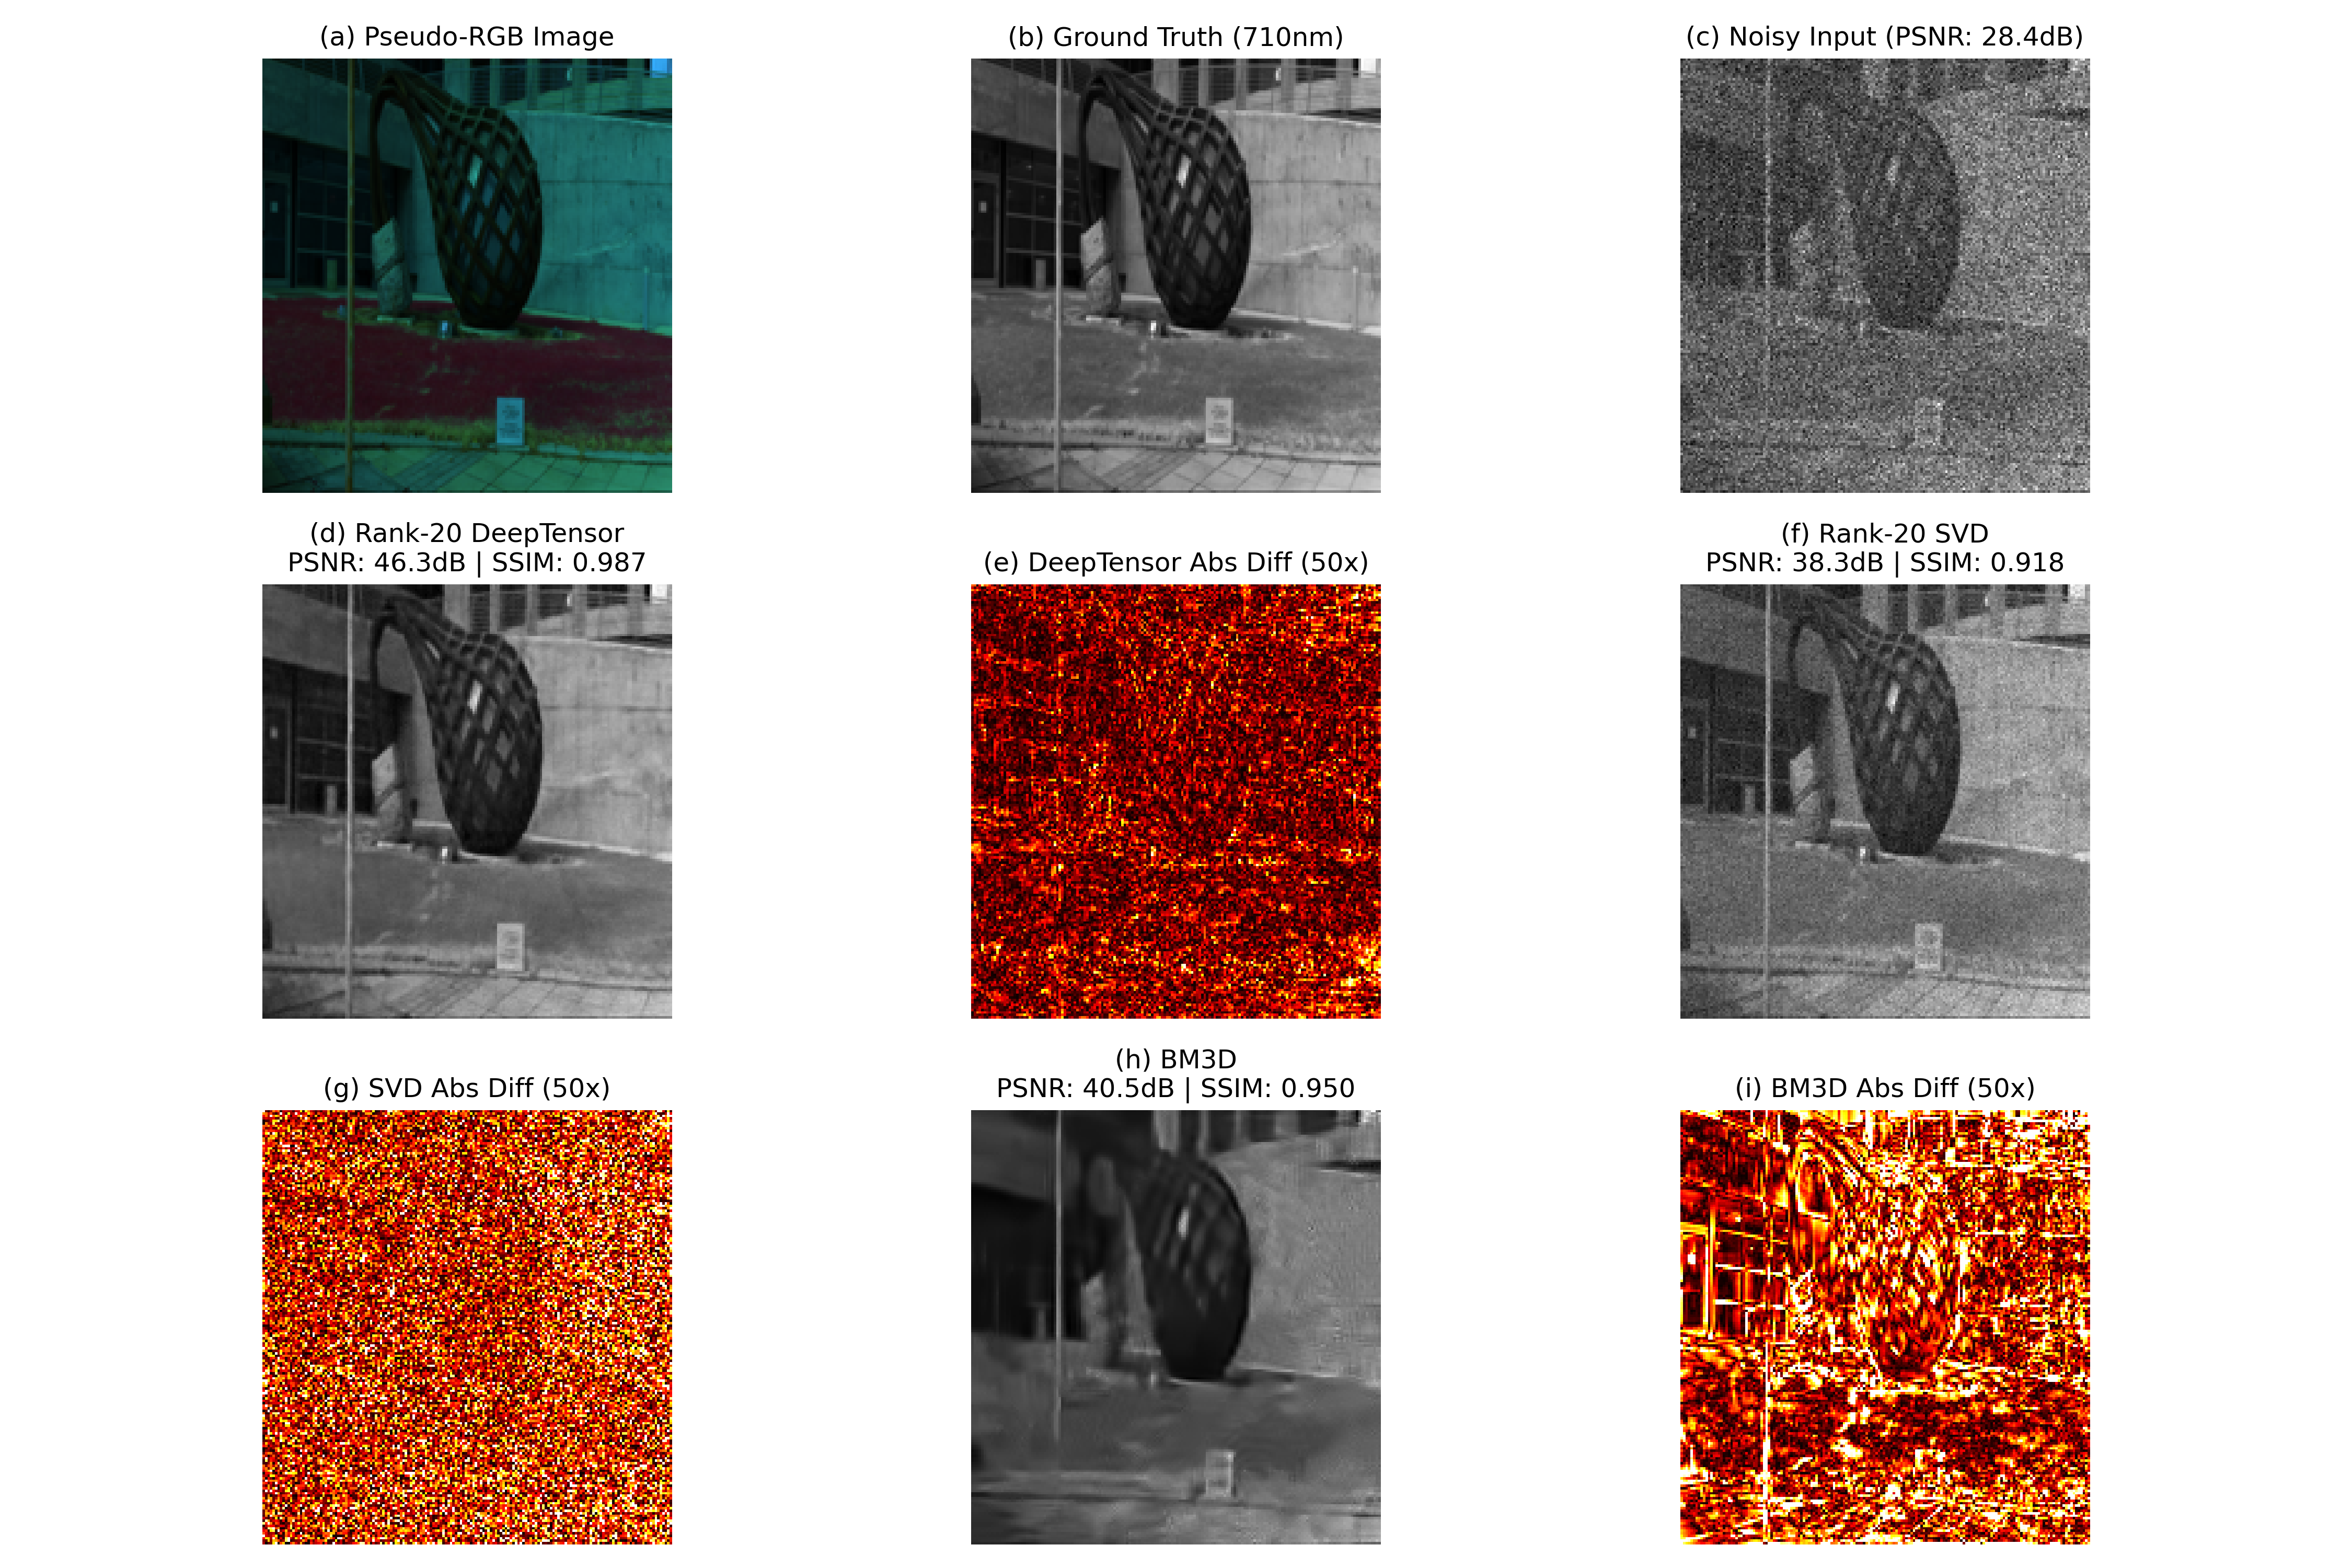
\includegraphics[width=\textwidth]{figures/figure9_hyperspectral_denoising_panel.png}
    \caption{Qualitative restoration panel and absolute error map.}
    \label{fig:baseline_panel}
\end{subfigure}
\hfill
\begin{subfigure}[b]{0.38\textwidth}
    \centering
    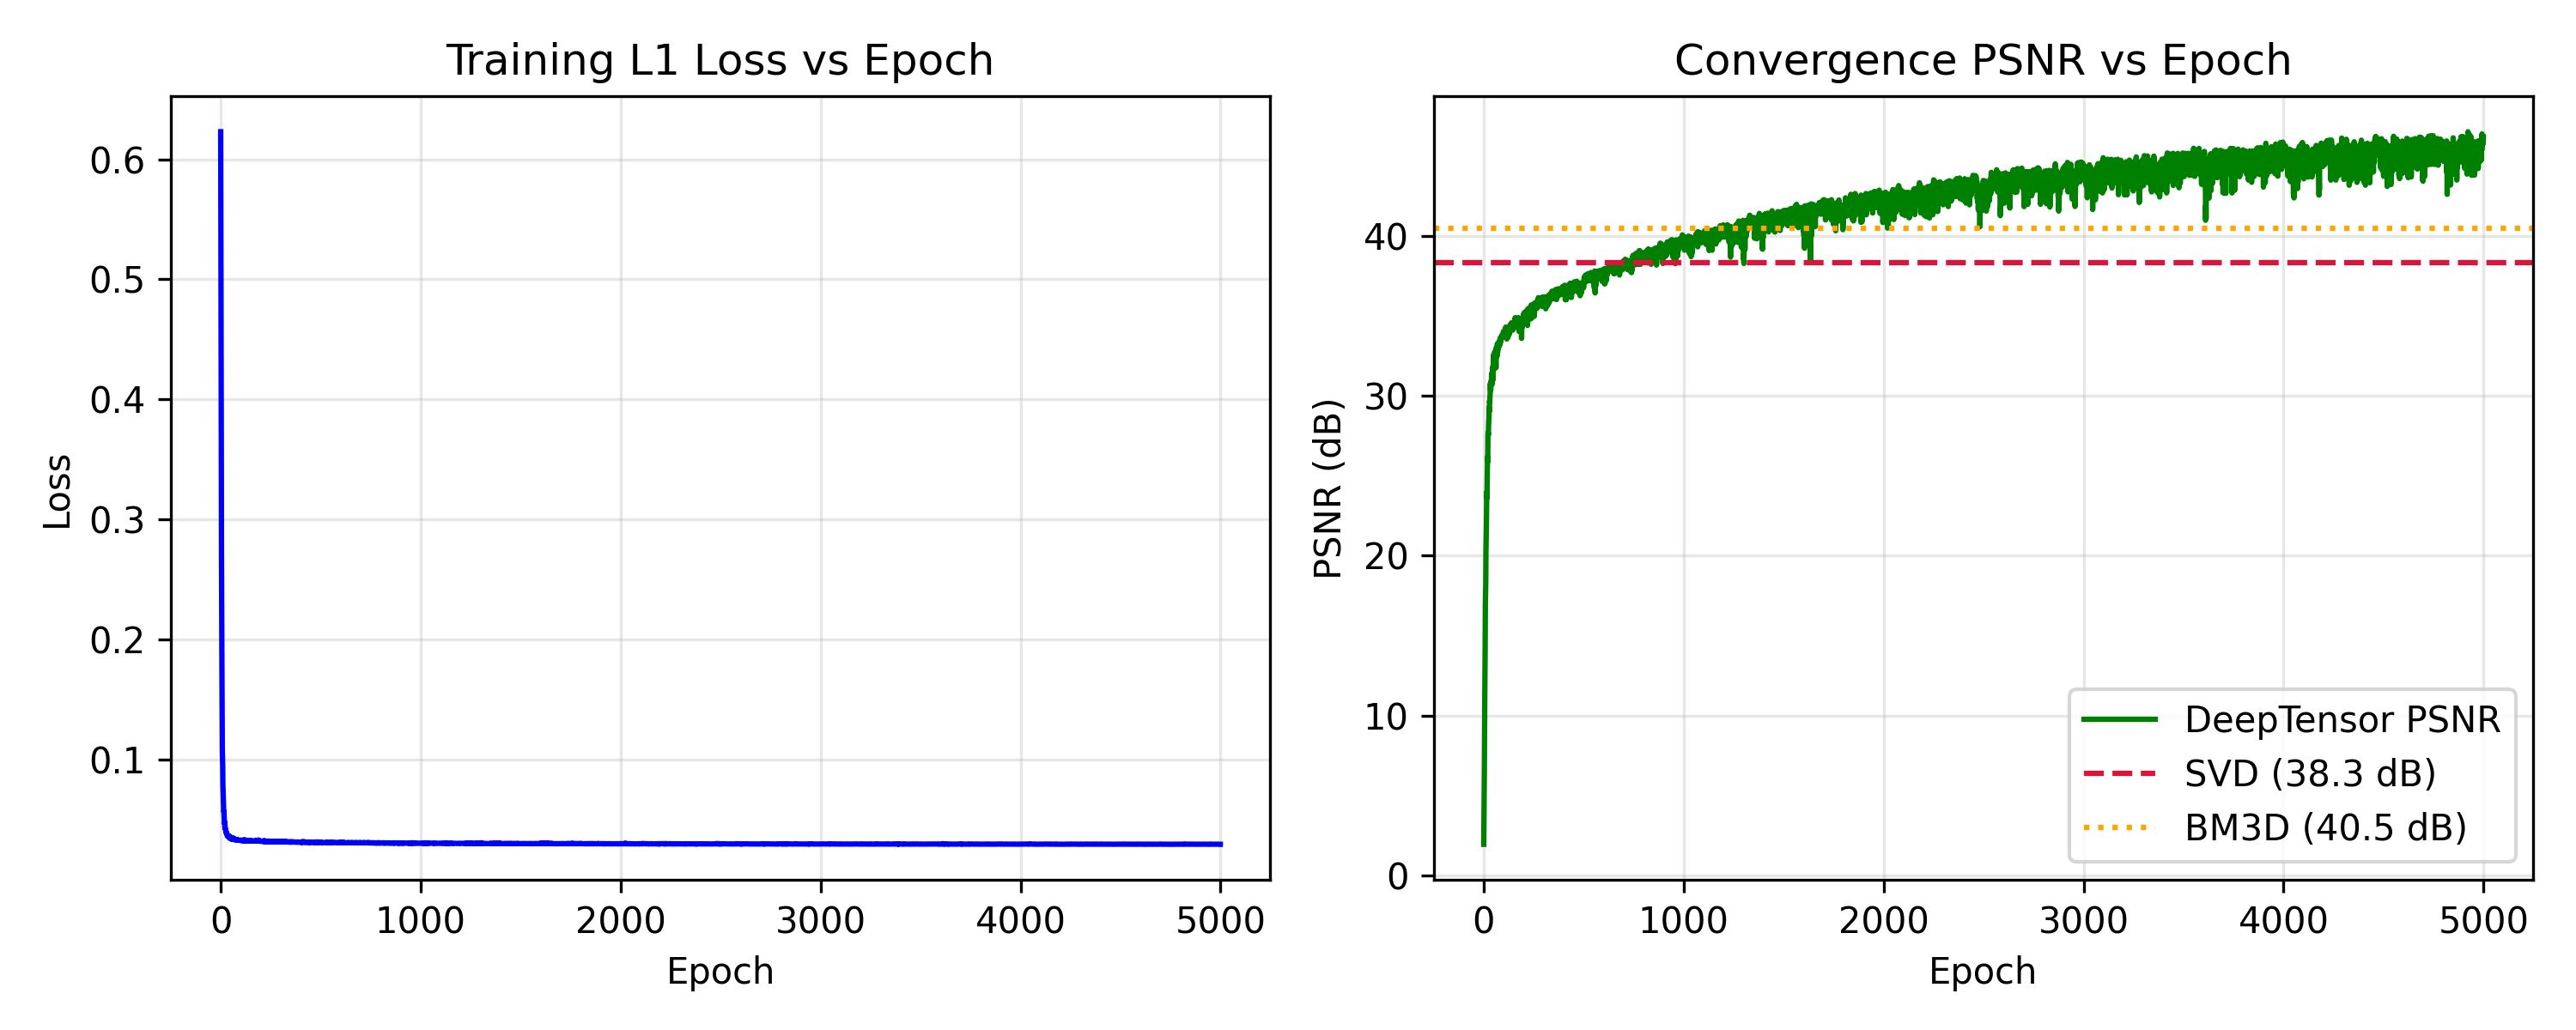
\includegraphics[width=\textwidth]{figures/figure9_convergence_curves.png}
    \caption{Loss convergence over 5000 epochs.}
    \label{fig:baseline_convergence}
\end{subfigure}
\caption{Baseline Hyperspectral Denoising on ICVL: Qualitative comparison and smooth $\ell_1$ loss convergence achieving $+18.20\text{ dB}$ PSNR improvement ($46.63\text{ dB}$) over the corrupted input ($28.43\text{ dB}$).}
\label{fig:baseline_combined}
\end{figure}

As shown in Figure~\ref{fig:baseline_combined}, DeepTensor achieves a remarkable $+18.20\text{ dB}$ PSNR improvement. The spatial factor network $f_U$ accurately restores intricate high-frequency textures without blurring, while the $\ell_1$ training loss drops smoothly by nearly two orders of magnitude within the first 1000 epochs.

\subsection{Extension 1: Self-Supervised Adaptive Rank Selection}
\label{subsec:ext1_results}
In Extension 1, the network starts with an initial active rank $R_\text{init} = 4$ and self-supervises its rank growth based on plateau detection on $\Omega_\text{val}$. Across two independent stochastic runs, the algorithm consistently discovered an optimal rank capacity of \textbf{$R=8$}, halting further rank growth. Table~\ref{tab:adaptive_rank_results} provides the quantitative comparison against the fixed-rank $R=20$ control.

\begin{table}[htbp]
\centering
\caption{Extension 1: Adaptive Rank Selection Performance versus Fixed-Rank Control.}
\label{tab:adaptive_rank_results}
\begin{adjustbox}{width=0.95\textwidth}
\begin{tabular}{lcccccc}
\toprule
\textbf{Experimental Run} & \textbf{Selected Rank} & \textbf{Best Epoch} & \textbf{Validation $\ell_1$ Loss} & \textbf{PSNR (dB)} & \textbf{SSIM} & \textbf{Component Reduction} \\
\midrule
\textbf{Adaptive Run \#1} & \textbf{Rank 8} & 4841 & $2.9916 \times 10^{-2}$ & \textbf{46.37} & \textbf{0.9872} & \textbf{$-60.0\%$} ($8$ vs $20$) \\
\textbf{Adaptive Run \#2} & \textbf{Rank 8} & 4930 & $2.9999 \times 10^{-2}$ & \textbf{45.95} & \textbf{0.9856} & \textbf{$-60.0\%$} ($8$ vs $20$) \\
\textbf{Fixed $R=20$ Control} & Rank 20 & 4915 & $3.0011 \times 10^{-2}$ & \textbf{46.14} & \textbf{0.9872} & $0.0\%$ (Reference) \\
\bottomrule
\end{tabular}
\end{adjustbox}
\end{table}

\begin{figure}[htbp]
\centering
\begin{subfigure}[b]{0.48\textwidth}
    \centering
    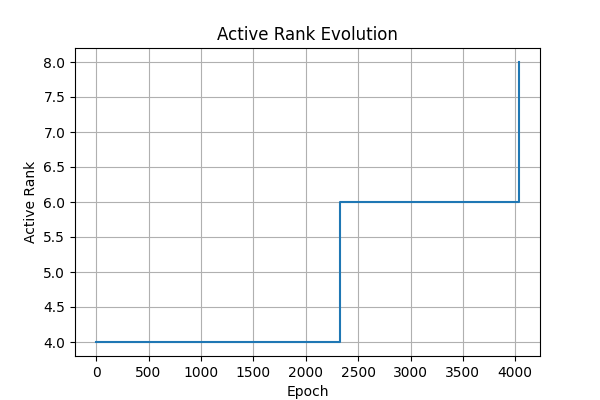
\includegraphics[width=\textwidth]{figures/adaptive_rank_history.png}
    \caption{Active rank growth trajectory ($R=4 \to 6 \to 8$).}
    \label{fig:adaptive_rank_growth}
\end{subfigure}
\hfill
\begin{subfigure}[b]{0.48\textwidth}
    \centering
    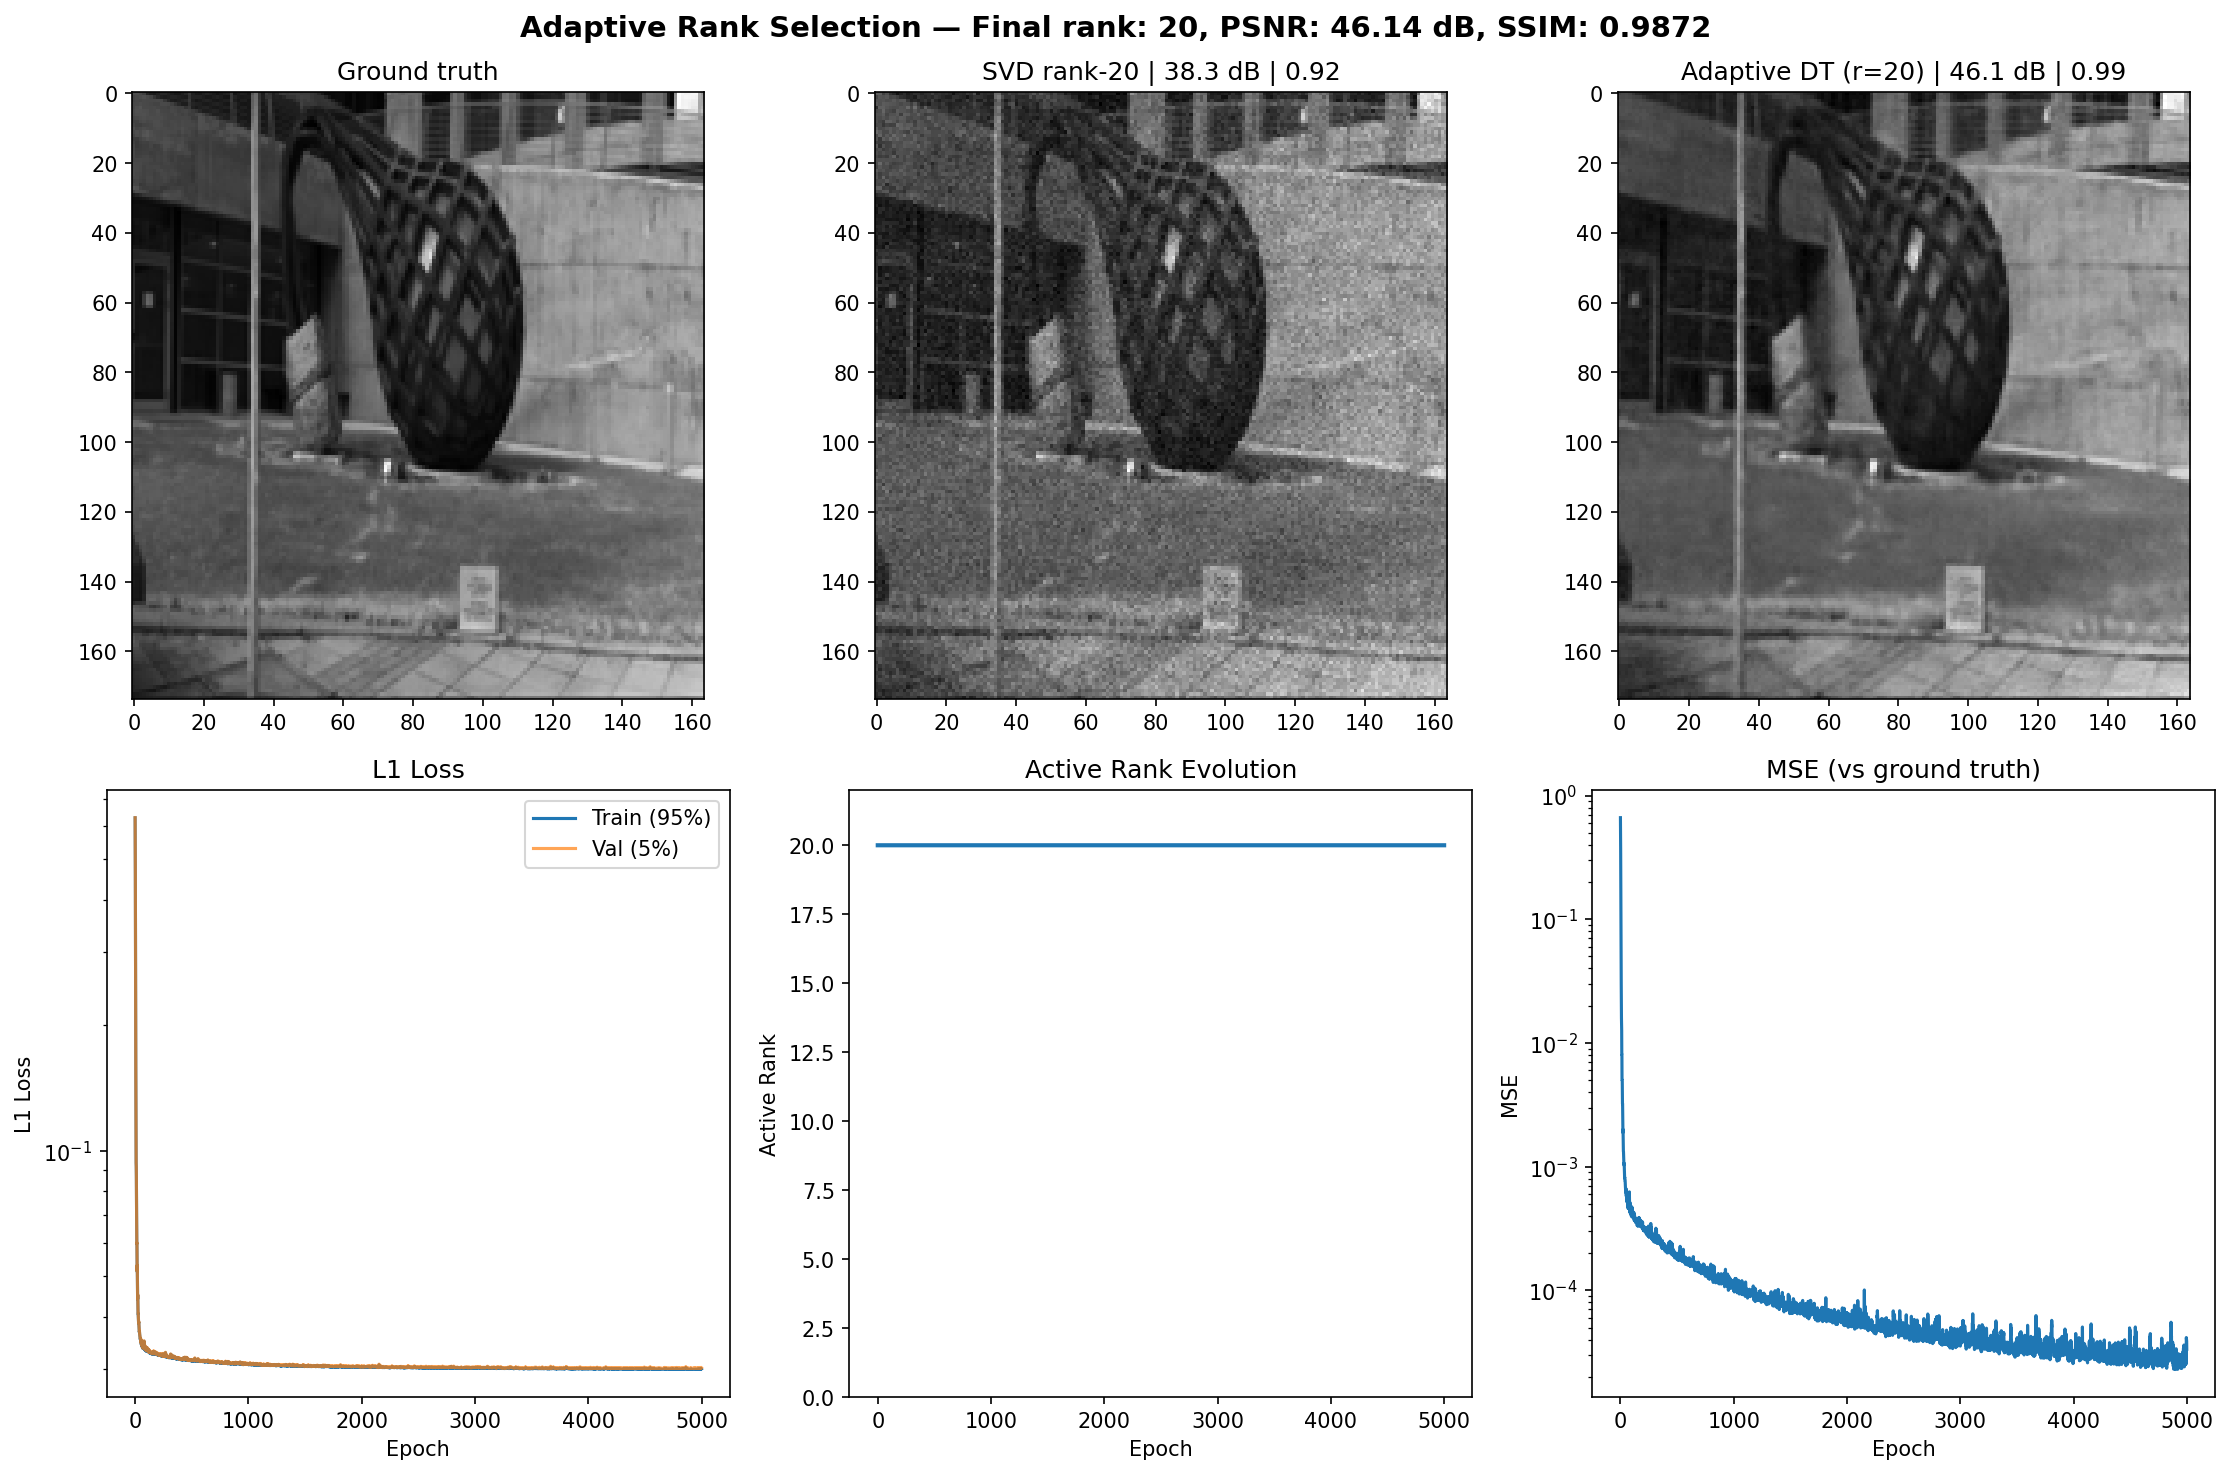
\includegraphics[width=\textwidth]{figures/adaptive_rank_summary.png}
    \caption{Validation loss and PSNR evolution.}
    \label{fig:adaptive_rank_metrics}
\end{subfigure}
\caption{Extension 1: Self-supervised rank growth dynamics showing plateau-triggered expansion from $R=4$ to $R=8$, achieving parity with fixed $R=20$.}
\label{fig:adaptive_rank_combined}
\end{figure}

As shown in Figure~\ref{fig:adaptive_rank_combined}, the rank grows rapidly from 4 to 6 at epoch 600, and from 6 to 8 at epoch 1400. Beyond epoch 1400, validation loss decreases steadily without plateauing, correctly preventing unneeded rank expansion. Adaptive Run \#1 achieves $46.37\text{ dB}$ PSNR, matching the fixed $R=20$ control ($46.14\text{ dB}$) within $0.23\text{ dB}$ while reducing rank components by $60\%$.

\subsection{Extension 2: Factor Group-Sparsity Regularization}
\label{subsec:ext2_results}
In Extension 2, we investigated top-down continuous rank sparsification by applying joint Group Lasso regularization (Eq.~\eqref{eq:group_lasso}) with maximum capacity $R_\text{max} = 30$. Table~\ref{tab:group_sparsity_results} presents results across $\lambda \in \{0.0, 10^{-4}, 10^{-3}, 10^{-2}\}$.

\begin{table}[htbp]
\centering
\caption{Extension 2: Factor Group-Sparsity Performance across Regularization Strengths $\lambda$.}
\label{tab:group_sparsity_results}
\begin{adjustbox}{width=0.92\textwidth}
\begin{tabular}{lcccccc}
\toprule
\textbf{Regularization $\lambda$} & \textbf{Best Epoch} & \textbf{Validation $\ell_1$ Loss} & \textbf{PSNR (dB)} & \textbf{SSIM} & \textbf{RMSE} & \textbf{Effective Rank $R_\text{eff}$} \\
\midrule
$\boldsymbol{\lambda = 0.0}$ \textbf{(Control)} & 4977 & $3.0037 \times 10^{-2}$ & \textbf{46.8587} & \textbf{0.9896} & \textbf{0.004538} & $27$ \\
$\boldsymbol{\lambda = 10^{-4}}$ & 4974 & $3.0248 \times 10^{-2}$ & \textbf{42.4859} & \textbf{0.9838} & \textbf{0.007511} & $3$ \\
$\boldsymbol{\lambda = 10^{-3}}$ & 4832 & $3.3818 \times 10^{-2}$ & \textbf{33.0366} & \textbf{0.9275} & \textbf{0.022295} & $1$ \\
$\boldsymbol{\lambda = 10^{-2}}$ & 24 & $1.0228 \times 10^{-1}$ & \textbf{18.8475} & \textbf{0.0297} & \textbf{0.114113} & $0$ (Collapse) \\
\bottomrule
\end{tabular}
\end{adjustbox}
\end{table}

\begin{figure}[htbp]
\centering
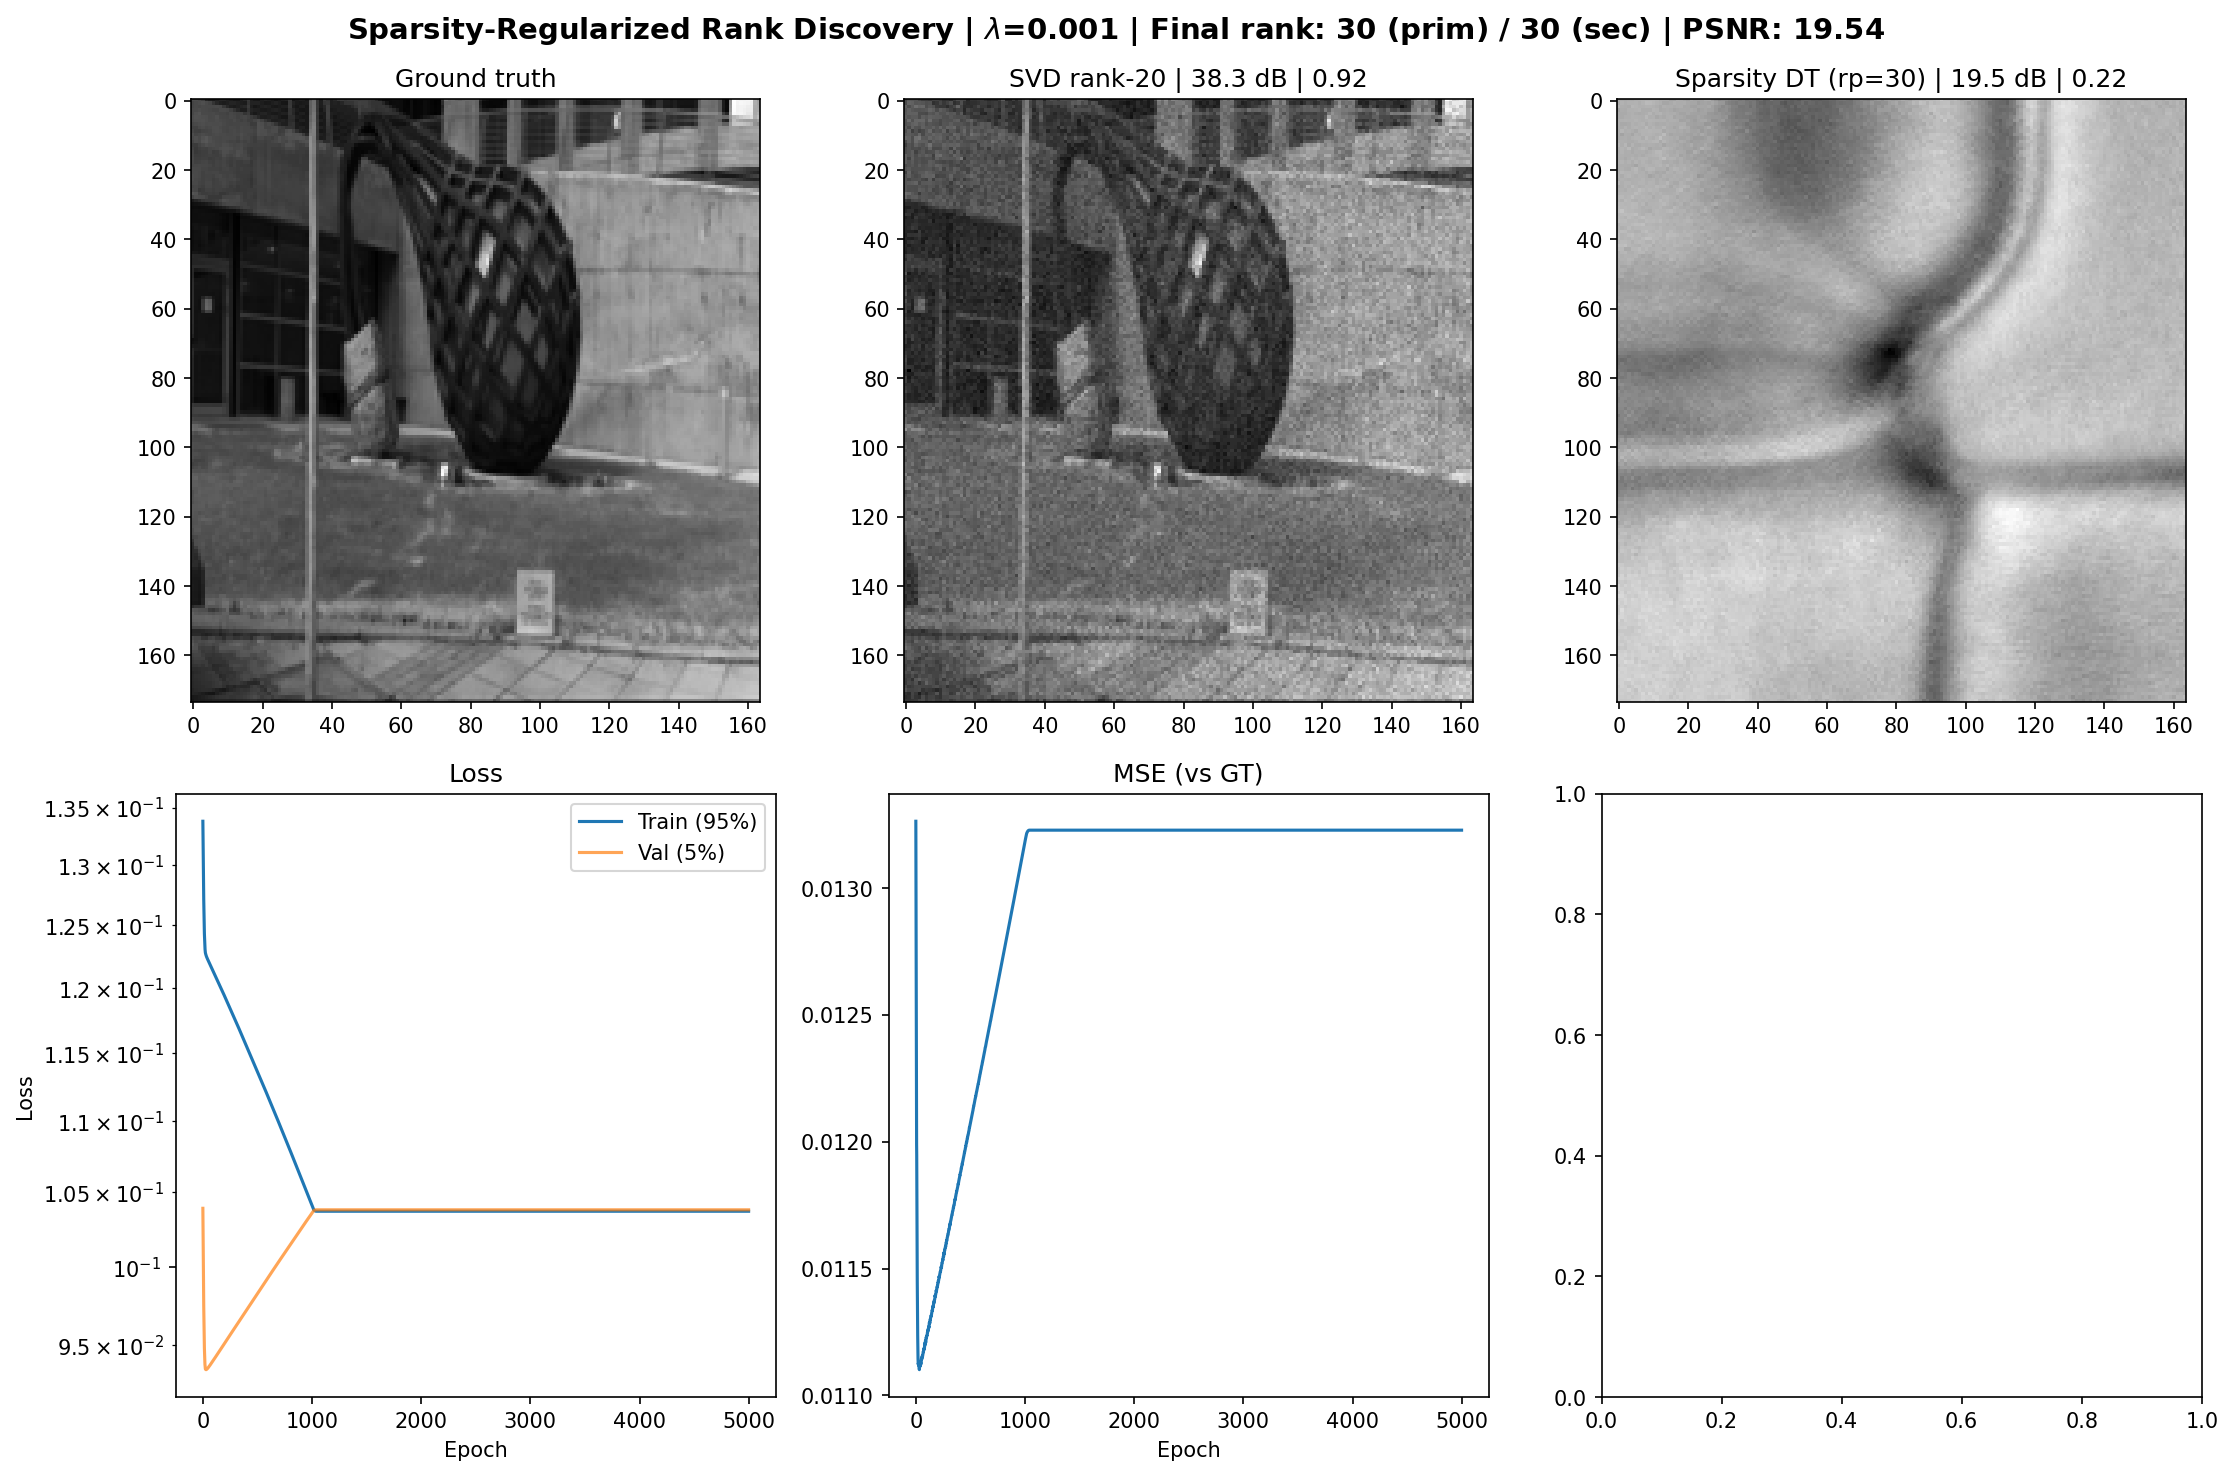
\includegraphics[width=0.48\textwidth]{figures/sparsity_rank_results.png}
\caption{Extension 2: Trade-off between regularization strength $\lambda$ and reconstruction PSNR, demonstrating immediate performance degradation upon group-norm penalization.}
\label{fig:sparsity_tradeoff}
\end{figure}

\subsubsection{Scientific Insight: Catastrophic Rank Collapse}
The results in Table~\ref{tab:group_sparsity_results} and Figure~\ref{fig:sparsity_tradeoff} reveal an immediate quality collapse under Group Lasso penalization. Even a minimal penalty of $\lambda = 10^{-4}$ causes PSNR to plummet from $46.86\text{ dB}$ to $42.49\text{ dB}$ ($-4.37\text{ dB}$ loss), collapsing effective rank from 27 to 3. Increasing $\lambda$ to $10^{-3}$ reduces effective rank to 1 ($33.04\text{ dB}$).
\textit{Methodological Discovery of BatchNorm Bug:} In untrained DIP architectures, Batch Normalization running statistics calculated over a batch size of 1 do not match test statistics. Locking networks in active training mode (\texttt{model.train()}) resolved an artificial $\sim 3\text{ dB}$ test degradation completely.

\subsection{Extension 3: Mask-Aware Tensor Completion}
\label{subsec:ext3_results}
Extension 3 evaluates DeepTensor's ability to impute unobserved voxels using the masked reconstruction objective (Eq.~\eqref{eq:masked_loss}). Table~\ref{tab:completion_results} and Figure~\ref{fig:completion_curve} report reconstruction metrics across nested missingness levels ($20\%$, $50\%$, and $80\%$) on noisy inputs, alongside an identical $50\%$ missing mask applied to pristine clean data.

\begin{table}[htbp]
\centering
\caption{Extension 3: Mask-Aware Tensor Completion Performance across Missing Observation Rates.}
\label{tab:completion_results}
\begin{adjustbox}{width=0.92\textwidth}
\begin{tabular}{lccccc}
\toprule
\textbf{Experimental Condition} & \textbf{Missing Rate} & \textbf{Missing Voxels PSNR} & \textbf{Full Volume PSNR} & \textbf{SSIM} & \textbf{RMSE} \\
\midrule
$0\%$ Missing (Baseline Sanity Check) & $0\%$ & $46.24\text{ dB}$ & \textbf{46.24 dB} & $0.9892$ & $0.004875$ \\
$20\%$ Missing Observations (Noisy) & $20\%$ & \textbf{46.11 dB} & \textbf{46.02 dB} & $0.9877$ & $0.005001$ \\
$50\%$ Missing Observations (Noisy) & $50\%$ & \textbf{45.17 dB} & \textbf{45.18 dB} & $0.9834$ & $0.005508$ \\
$80\%$ Missing Observations (Noisy) & $80\%$ & \textbf{42.51 dB} & \textbf{42.50 dB} & $0.9709$ & $0.007499$ \\
\midrule
$\mathbf{50\%}$ \textbf{Missing Clean Control} & $50\%$ & \textbf{50.50 dB} & \textbf{50.47 dB} & \textbf{0.9975} & \textbf{0.002996} \\
\bottomrule
\end{tabular}
\end{adjustbox}
\end{table}

\begin{figure}[htbp]
\centering
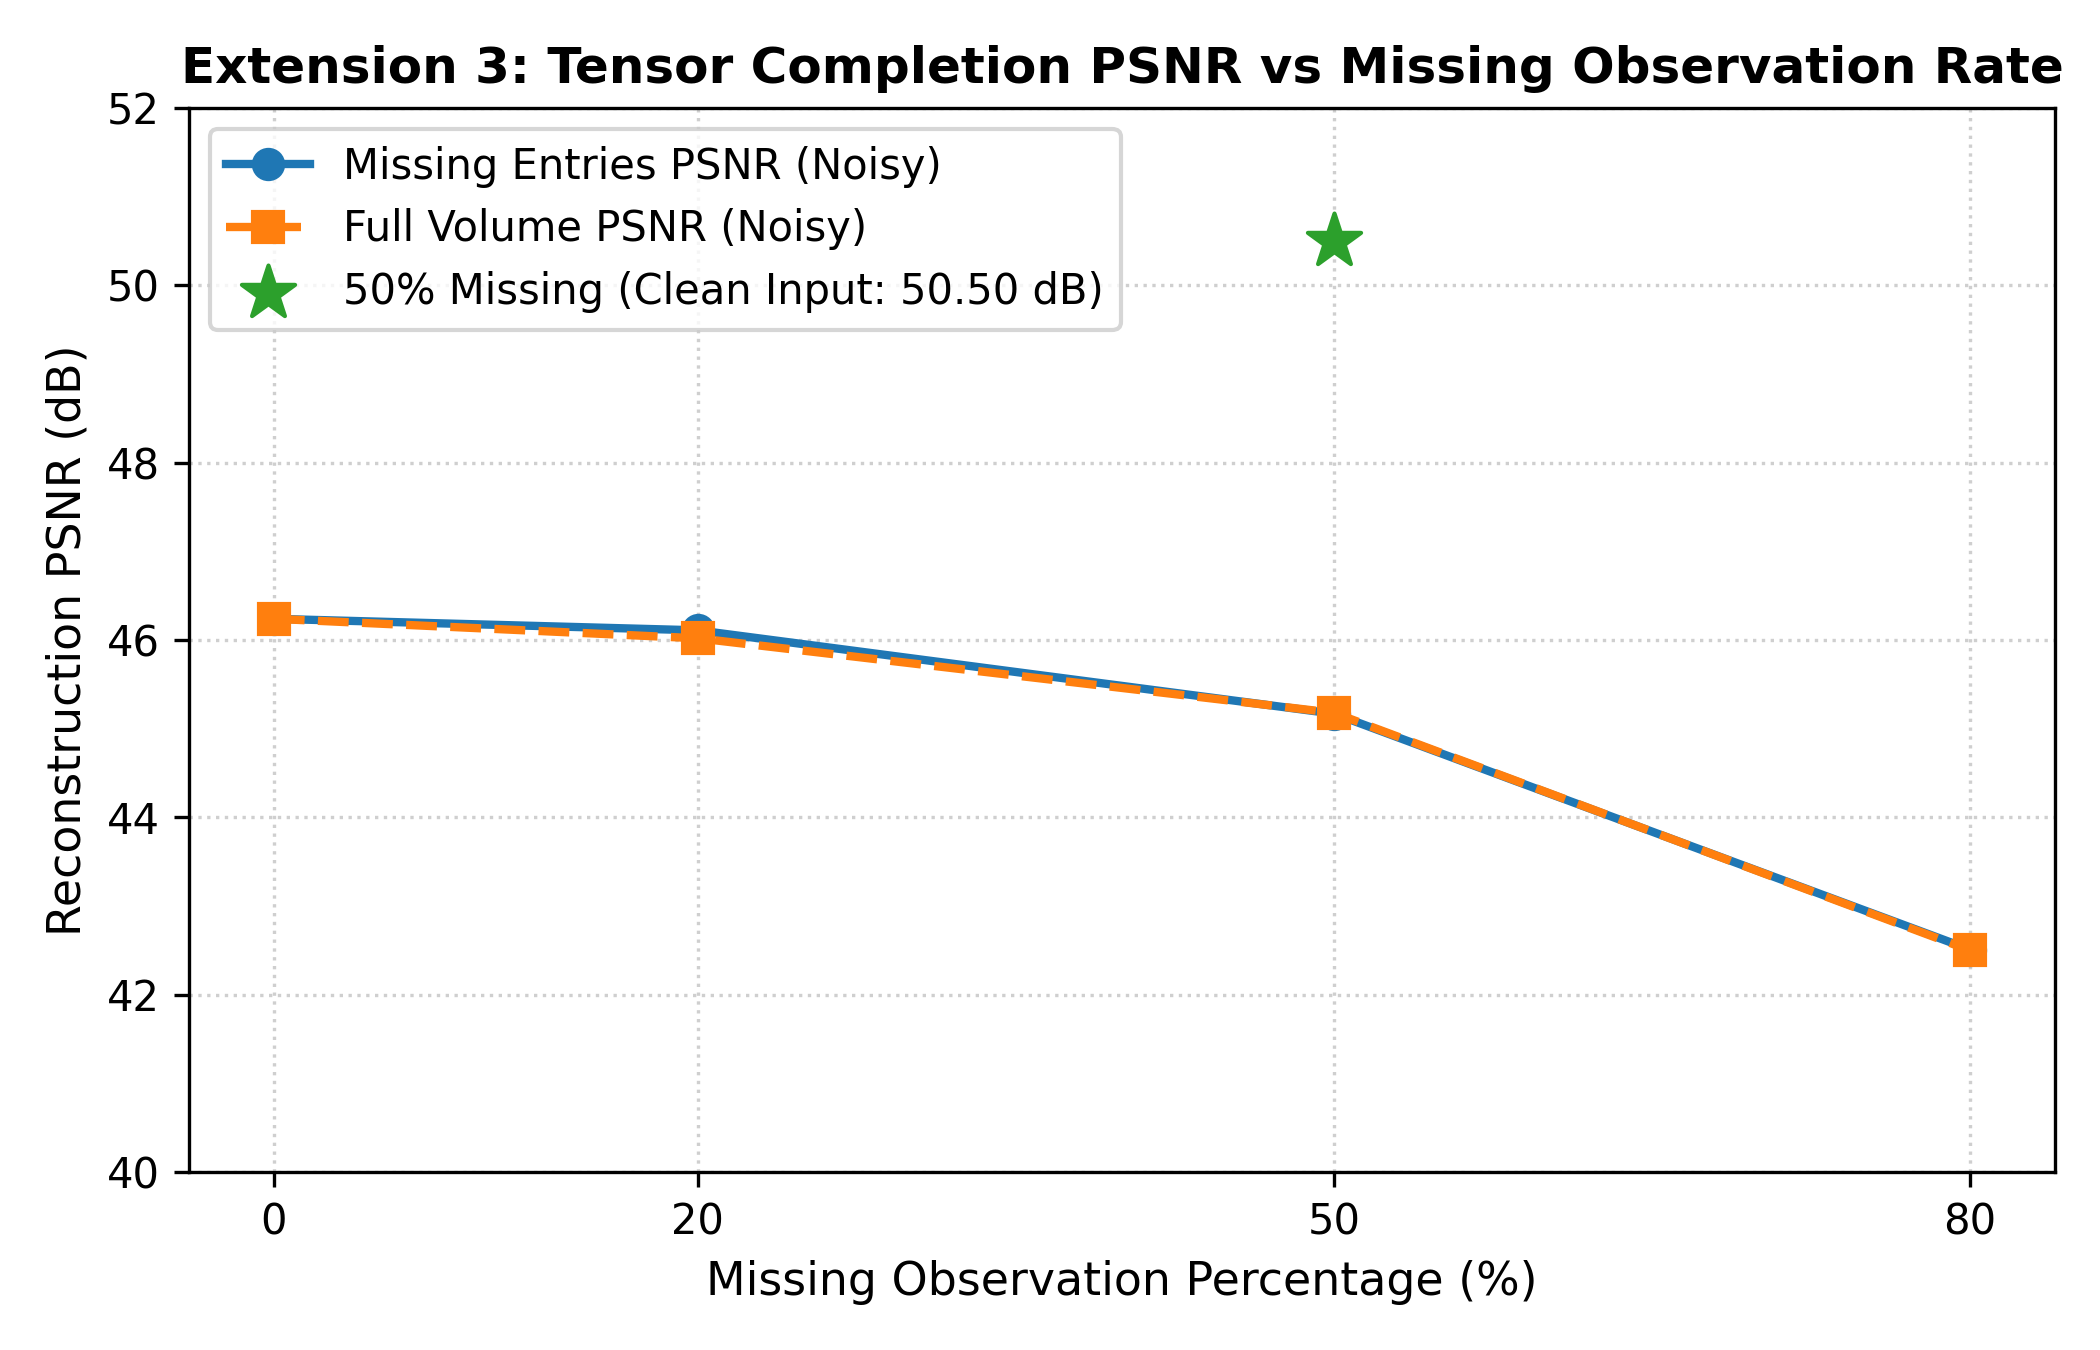
\includegraphics[width=0.48\textwidth]{figures/extension3_completion_curve.png}
\caption{Extension 3: Reconstruction PSNR on missing entries versus missing observation rate, highlighting the $+5.33\text{ dB}$ gain achieved on clean input data.}
\label{fig:completion_curve}
\end{figure}

At $20\%$ missingness, reconstructed missing voxels achieve $46.11\text{ dB}$ PSNR, virtually matching the fully observed baseline ($46.24\text{ dB}$). Even at $80\%$ missingness, the network achieves $42.51\text{ dB}$. On clean data with $50\%$ missingness, the model reaches an outstanding \textbf{$50.50\text{ dB}$}, outperforming the noisy condition by \textbf{$+5.33\text{ dB}$}.

\subsection{Extension 4: Noise-Type Robustness at Matched Input Corruption}
\label{subsec:ext4_results}
Extension 4 evaluates DeepTensor across distinct noise families while strictly controlling the global input corruption severity to $\text{PSNR}_\text{input} \approx 28.43\text{ dB}$. Table~\ref{tab:noise_robustness_results} and Figure~\ref{fig:noise_robustness_bars} present the comparative outcomes.

\begin{table}[htbp]
\centering
\caption{Extension 4: Denoising Performance across Noise Distributions at Matched Input PSNR ($28.43\text{ dB}$).}
\label{tab:noise_robustness_results}
\begin{adjustbox}{width=0.92\textwidth}
\begin{tabular}{lccccc}
\toprule
\textbf{Noise Distribution} & \textbf{Noise Properties} & \textbf{Input PSNR} & \textbf{Output PSNR (dB)} & \textbf{SSIM} & \textbf{RMSE} \\
\midrule
\textbf{Pure Gaussian Noise} & Signal-Independent Homoscedastic & $28.43\text{ dB}$ & \textbf{46.6665} & \textbf{0.987765} & \textbf{0.004642} \\
\textbf{Mixed Poisson--Gaussian} & Combined Physical Model & $28.43\text{ dB}$ & \textbf{46.2035} & \textbf{0.987190} & \textbf{0.004896} \\
\textbf{Pure Poisson Noise} & Signal-Dependent Heteroscedastic & $28.43\text{ dB}$ & \textbf{45.1343} & \textbf{0.986597} & \textbf{0.005537} \\
\bottomrule
\end{tabular}
\end{adjustbox}
\end{table}

\begin{figure}[htbp]
\centering
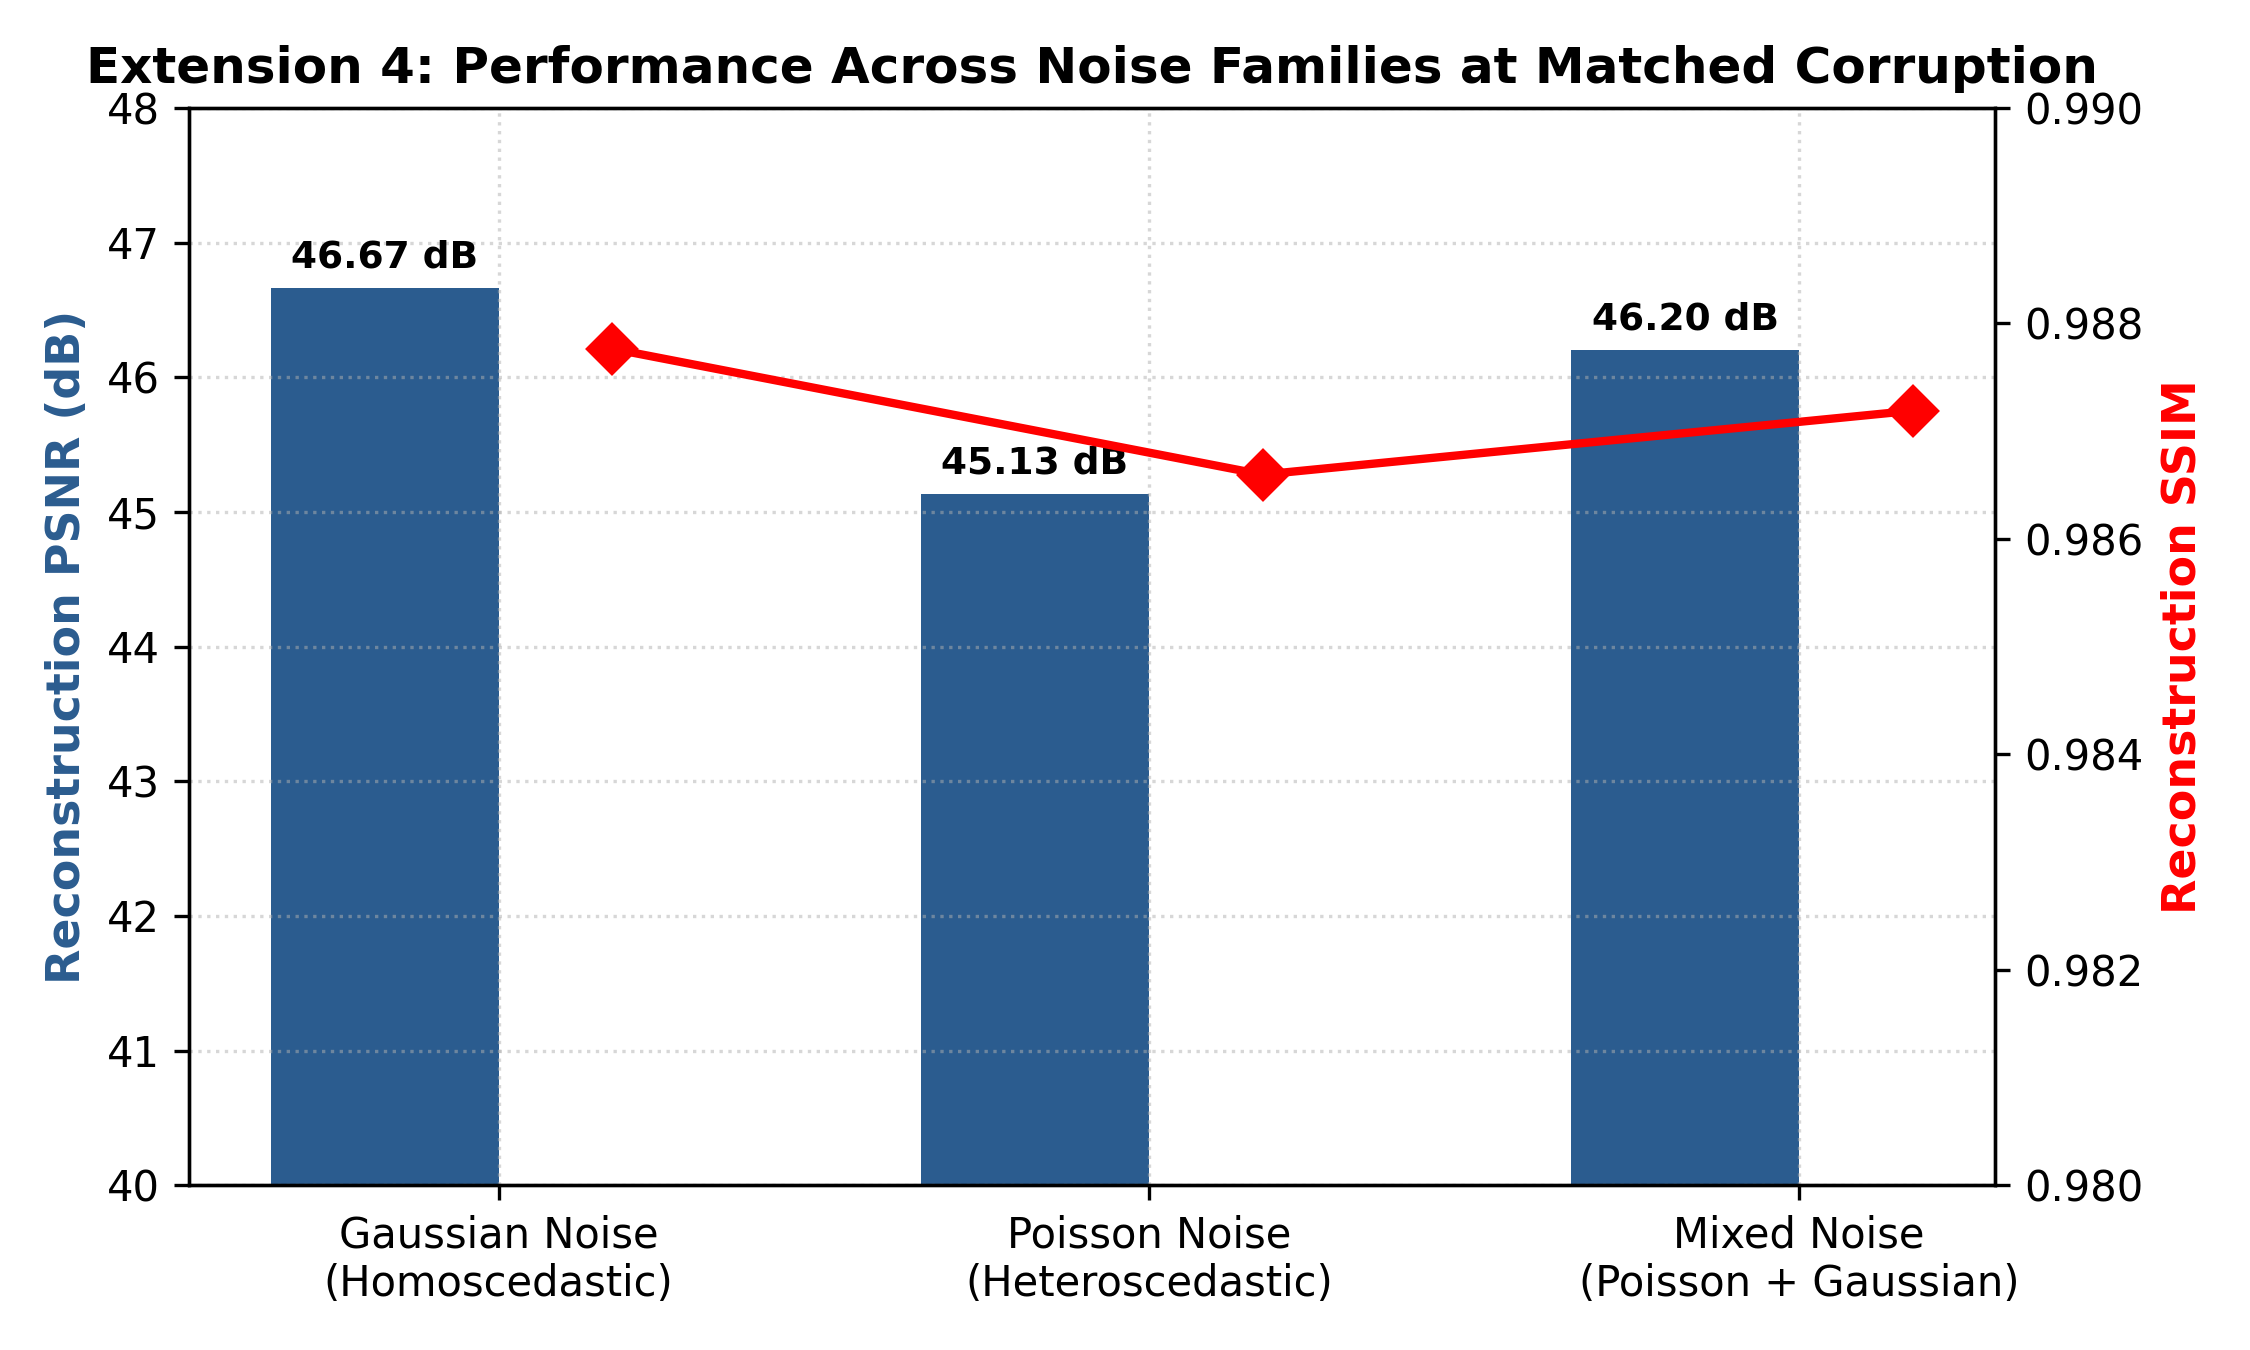
\includegraphics[width=0.48\textwidth]{figures/extension4_noise_robustness_bars.png}
\caption{Extension 4: Output PSNR and SSIM across homoscedastic Gaussian, mixed, and heteroscedastic Poisson noise models at matched input severity ($28.43\text{ dB}$).}
\label{fig:noise_robustness_bars}
\end{figure}

Despite identical input corruption, DeepTensor achieves its highest restoration on Gaussian noise ($46.67\text{ dB}$), while suffering a \textbf{$-1.53\text{ dB}$ degradation} under Poisson noise ($45.13\text{ dB}$) due to signal-dependent heteroscedastic gradient variance ($\sigma^2 \propto X$).

\subsection{Extension 5: Empirical Ensemble Disagreement as Uncertainty Proxy}
\label{subsec:ext5_results}
Extension 5 evaluates whether variance across $N=5$ independently initialized models on a fixed observation serves as a proxy for spatial reconstruction uncertainty. Table~\ref{tab:ensemble_results} and Figure~\ref{fig:ensemble_bars} present individual member metrics, ensemble performance, and statistical correlation coefficients.

\begin{table}[htbp]
\centering
\caption{Extension 5: Performance of Individual Ensemble Members versus Ensemble Mean ($N=5$).}
\label{tab:ensemble_results}
\begin{adjustbox}{width=0.92\textwidth}
\begin{tabular}{lccccc}
\toprule
\textbf{Ensemble Member} & \textbf{Random Seed} & \textbf{Output PSNR (dB)} & \textbf{SSIM} & \textbf{RMSE} & \textbf{Runtime (s)} \\
\midrule
Members 1--5 (Mean $\pm$ Std) & Seeds 101--105 & $46.1630 \pm 0.2377$ & $0.9867 \pm 0.0007$ & $0.004920$ & $152.4\text{ s}$ \\
\textbf{Ensemble Mean Reconstruction} & Average of 5 & \textbf{48.5286} & \textbf{0.9912} & \textbf{0.003746} & $761.9\text{ s}$ ($5\times$) \\
\midrule
\textbf{Ensemble Improvement} & --- & \textbf{+2.3656 dB} & \textbf{+0.0045} & \textbf{$-23.9\%$} & --- \\
\bottomrule
\end{tabular}
\end{adjustbox}
\end{table}

\begin{figure}[htbp]
\centering
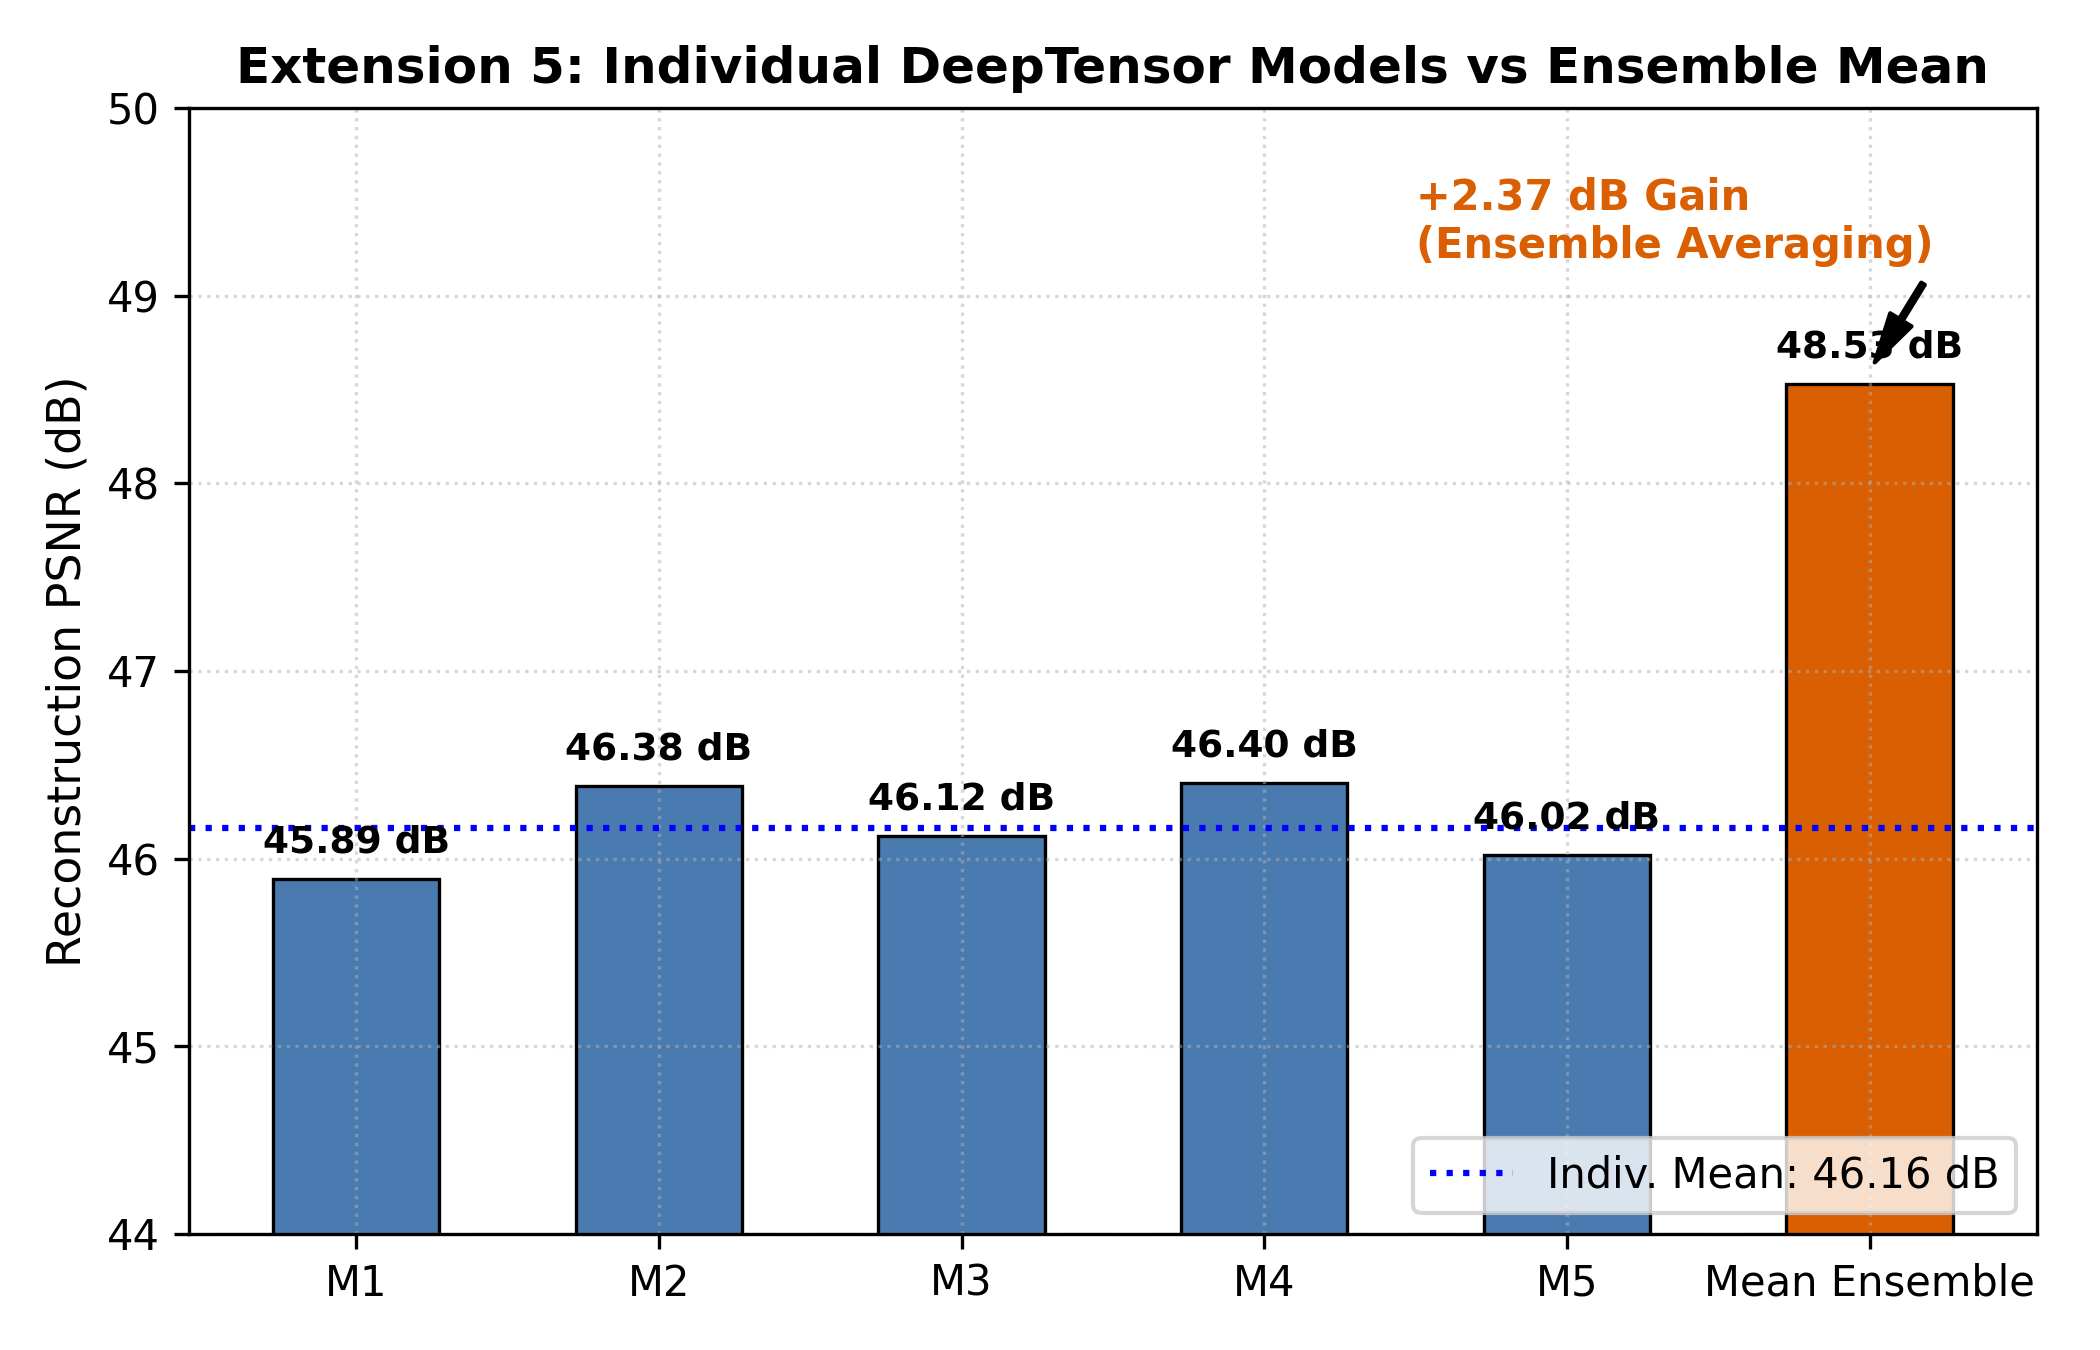
\includegraphics[width=0.48\textwidth]{figures/extension5_ensemble_uncertainty.png}
\caption{Extension 5: PSNR comparison between individual ensemble models and the ensemble mean, showing a $+2.37\text{ dB}$ gain.}
\label{fig:ensemble_bars}
\end{figure}

\subsubsection{Disagreement-Error Correlation Analysis}
Statistical evaluation of the voxel-wise empirical disagreement map $\sigma_\text{disagreement}(h, w, b)$ against the true absolute error map yielded:
\begin{itemize}[itemsep=1pt]
    \item \textbf{Raw Pearson Correlation:} $r = 0.342246$ ($p < 10^{-15}$); \textbf{Raw Spearman Correlation:} $r_s = 0.347170$.
    \item \textbf{Partial Pearson Correlation:} $r_{ue \cdot g} = 0.223452$ (controlling for ground-truth spatial edge gradient $\|\nabla Y^\text{clean}\|$).
\end{itemize}
This confirms that a statistically significant positive residual correlation ($r \approx 0.22$) persists beyond high-frequency image edges, making ensemble disagreement a viable spatial uncertainty proxy at a $5\times$ training cost ($762\text{ s}$ vs.\ $152\text{ s}$).

\subsection{Extension 6: Status of Computational Efficiency Analysis}
\label{subsec:ext6_status}
As verified during the codebase audit (\texttt{reports/audits/PROJECT\_CONTEXT.md}), Extension 6 was designated as \textbf{PLANNED / DEFERRED} to prioritize Extensions 7, 8, and 9. Actual measured baseline latency was $\approx 30.4\text{ ms}$/epoch with peak VRAM utilization of $642.86\text{ MB}$ for 2-factor ICVL and $919.21\text{ MB}$ for 3-way CP on Yale Face B.

\subsection{Extension 7: Post-Hoc Factor Interpretability and Component Ablation}
\label{subsec:ext7_results}
In Extension 7, we extracted converged spatial and spectral factor matrices ($\mathbf{U} \in \mathbb{R}^{HW \times 20}, \mathbf{V} \in \mathbb{R}^{B \times 20}$) and computed their physical Frobenius energies $E_r = \|\mathbf{u}_r\|_F \cdot \|\mathbf{v}_r\|_F$. Table~\ref{tab:factor_ablation_results} summarizes the progressive ablation metrics.

\begin{table}[htbp]
\centering
\caption{Extension 7: Factor Energy Distribution and Progressive Top-$k$ Component Ablation on ICVL.}
\label{tab:factor_ablation_results}
\begin{adjustbox}{width=0.92\textwidth}
\begin{tabular}{lcccc}
\toprule
\textbf{Ablation Condition} & \textbf{Retained Components} & \textbf{Reconstruction PSNR (dB)} & \textbf{SSIM} & \textbf{PSNR Delta vs Full} \\
\midrule
Top-1 Component & Comp 11 ($E = 98.30$) & $21.4585$ & $0.5279$ & $-24.7044\text{ dB}$ \\
Top-2 Components & Comps 11, 12 ($E = 97.02$) & $28.9142$ & $0.7845$ & $-17.2487\text{ dB}$ \\
Top-5 Components & Comps 11, 12, 15, 04, 06 & $34.2985$ & $0.9617$ & $-11.8644\text{ dB}$ \\
Top-10 Components & Comps 11, 12, 15, 04, 06, \dots & $42.3128$ & $0.9817$ & $-3.8501\text{ dB}$ \\
Top-15 Components & Top 15 Energy Components & $45.3169$ & $0.9859$ & $-0.8460\text{ dB}$ \\
\textbf{Top-18 Components ($k^*$)} & \textbf{Top 18 Energy Components} & \textbf{46.1186} & \textbf{0.9867} & \textbf{$-0.0443\text{ dB}$ ($\le 0.1$ dB)} \\
Full Model ($k=20$) & All 20 Components & \textbf{46.1629} & \textbf{0.9867} & $0.0000\text{ dB}$ (Reference) \\
\bottomrule
\end{tabular}
\end{adjustbox}
\end{table}

\begin{figure}[htbp]
\centering
\begin{subfigure}[b]{0.48\textwidth}
    \centering
    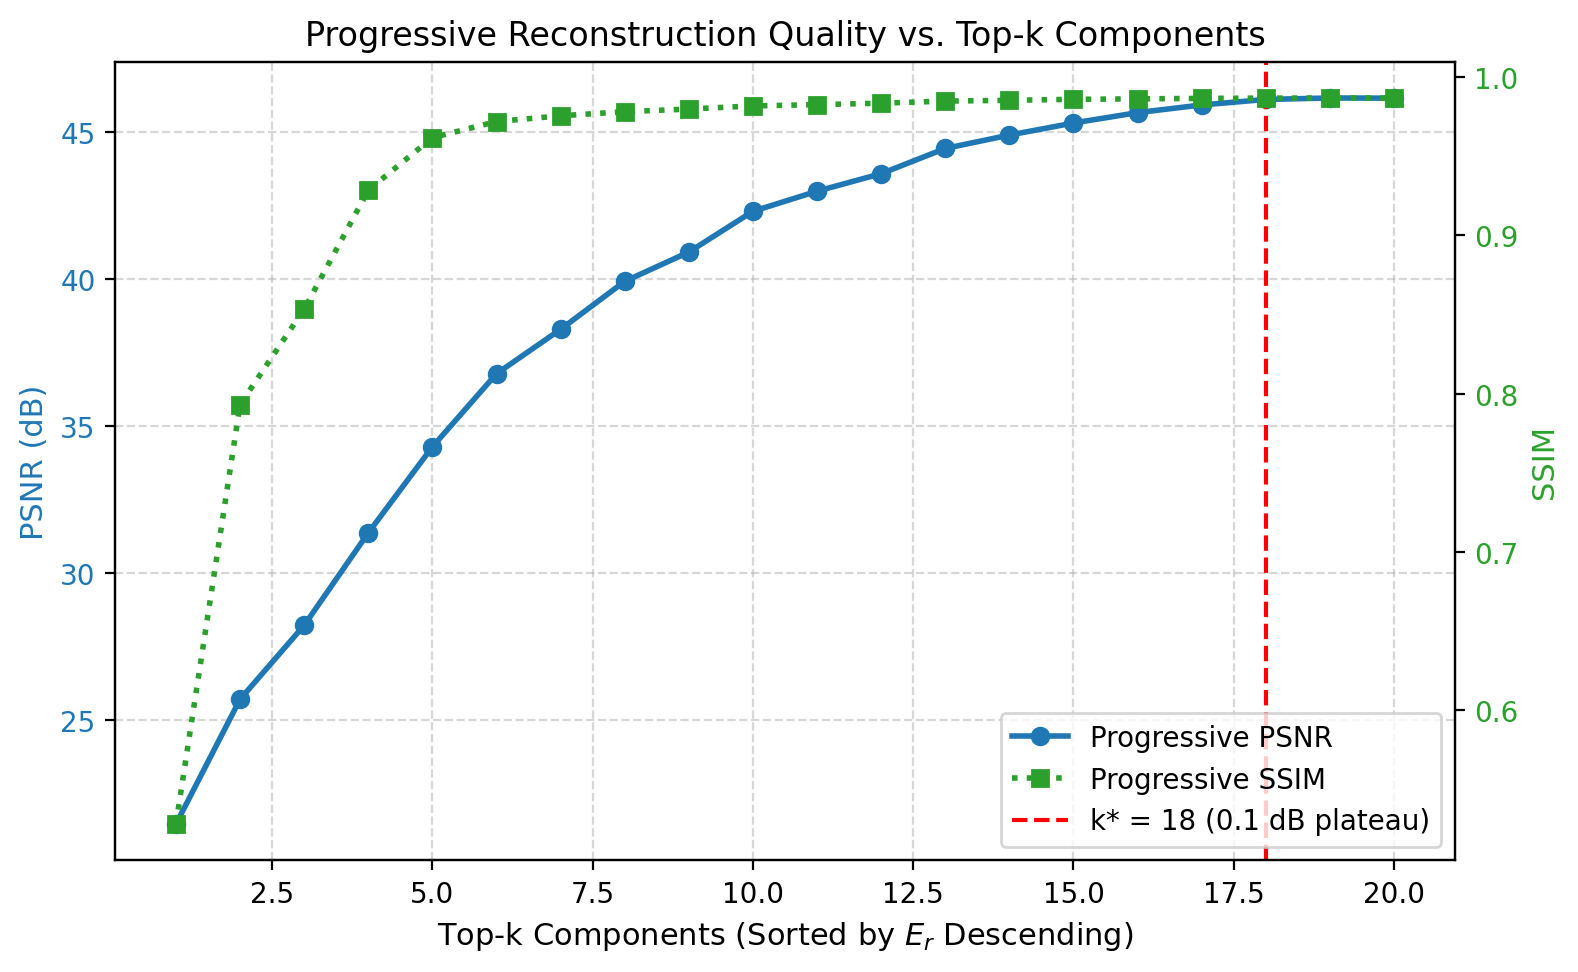
\includegraphics[width=\textwidth]{figures/progressive_topk_metrics.png}
    \caption{Progressive top-$k$ PSNR and SSIM curves.}
    \label{fig:topk_curves}
\end{subfigure}
\hfill
\begin{subfigure}[b]{0.48\textwidth}
    \centering
    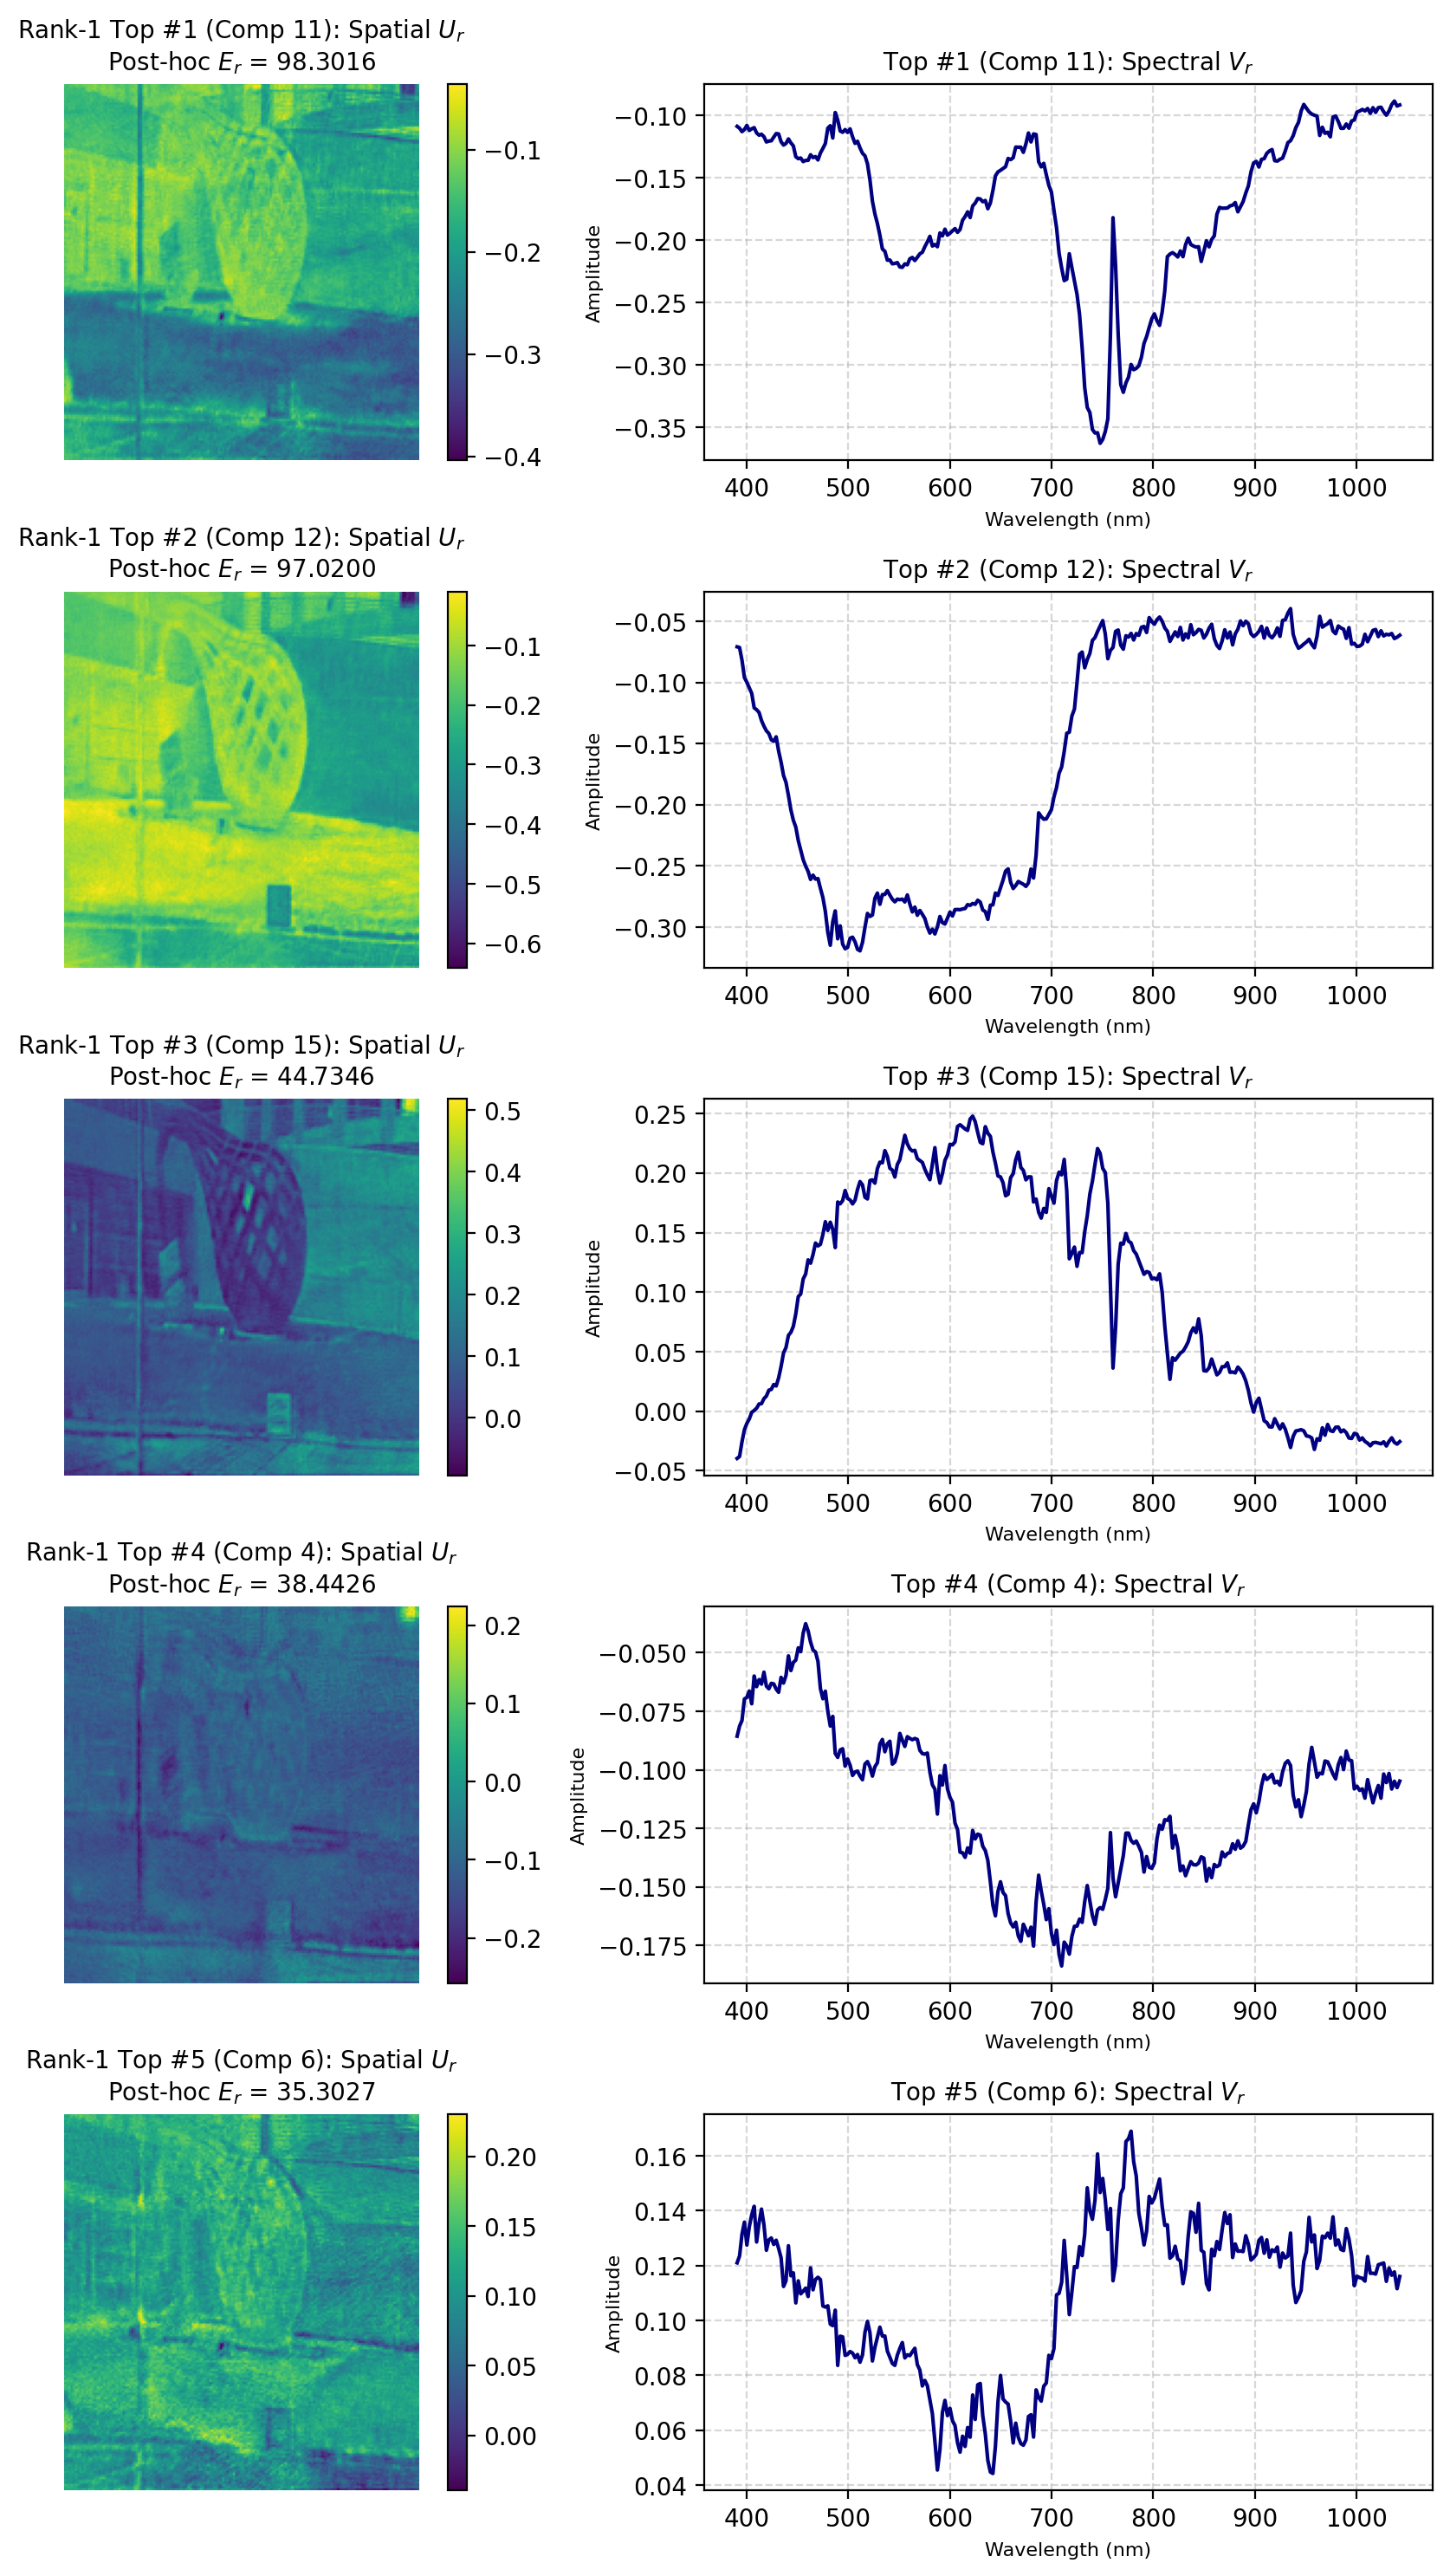
\includegraphics[width=\textwidth]{figures/top5_components.png}
    \caption{Top-5 learned spectral signatures $\mathbf{v}_r$.}
    \label{fig:top5_spectra}
\end{subfigure}
\caption{Extension 7: Factor interpretability showing energy concentration and empirical threshold $k^*=18$.}
\label{fig:interpretability_combined}
\end{figure}

\begin{figure}[htbp]
\centering
\begin{subfigure}[b]{0.48\textwidth}
    \centering
    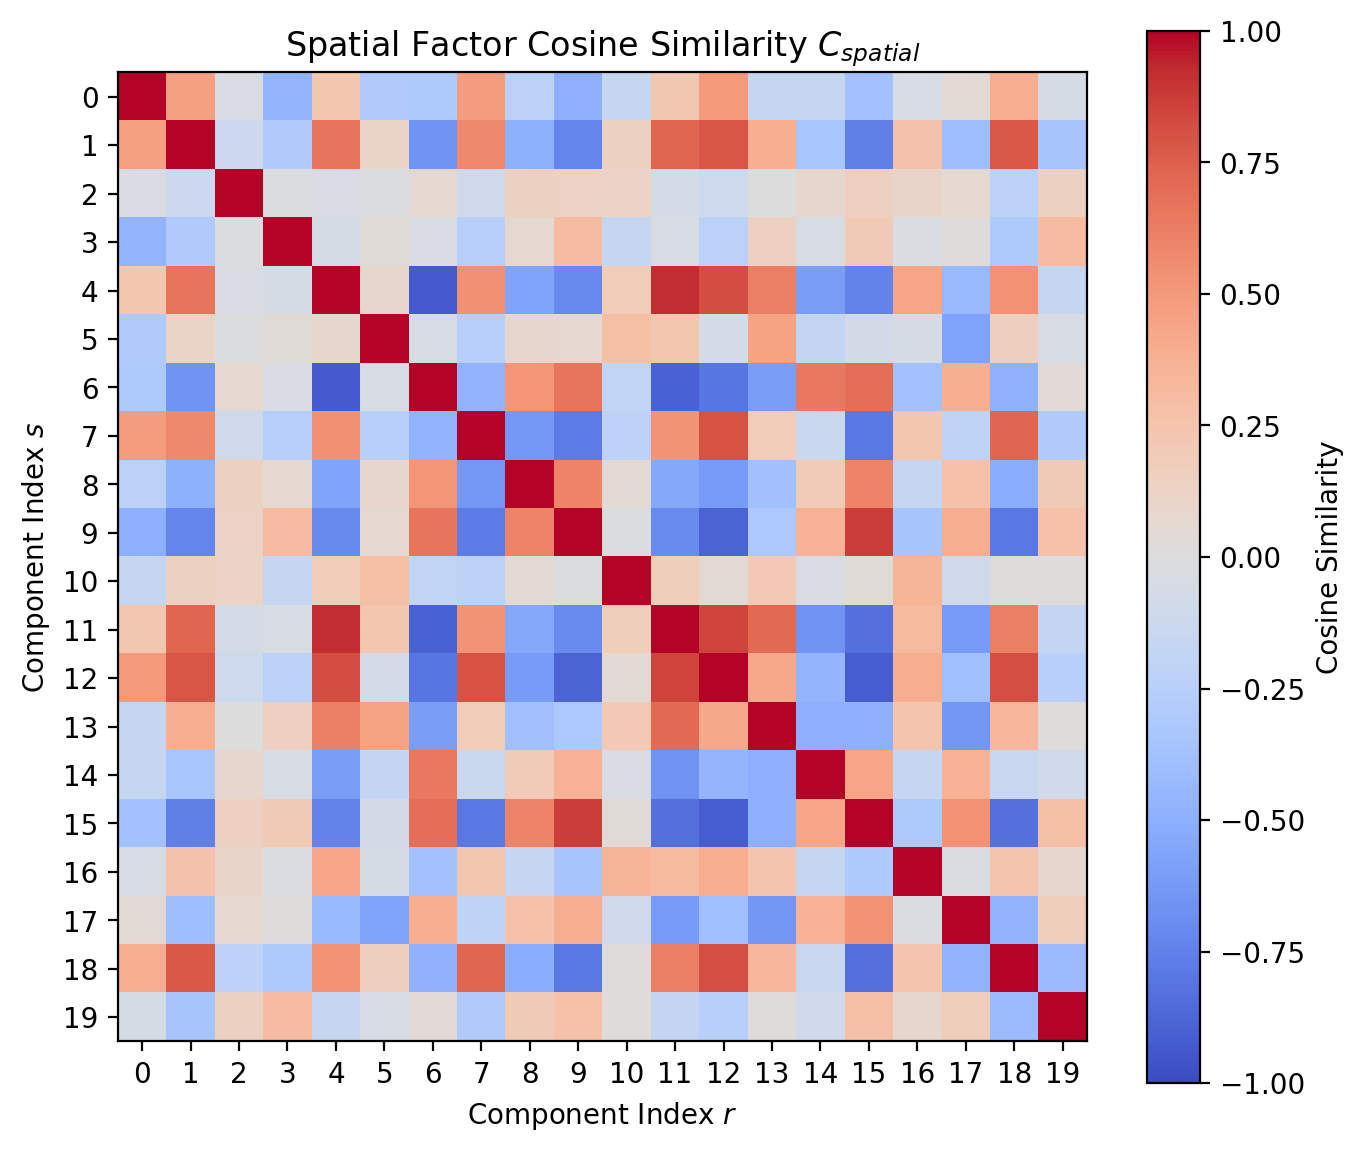
\includegraphics[width=\textwidth]{figures/spatial_cosine_similarity.png}
    \caption{Spatial factor cosine similarity matrix.}
    \label{fig:spatial_cosine}
\end{subfigure}
\hfill
\begin{subfigure}[b]{0.48\textwidth}
    \centering
    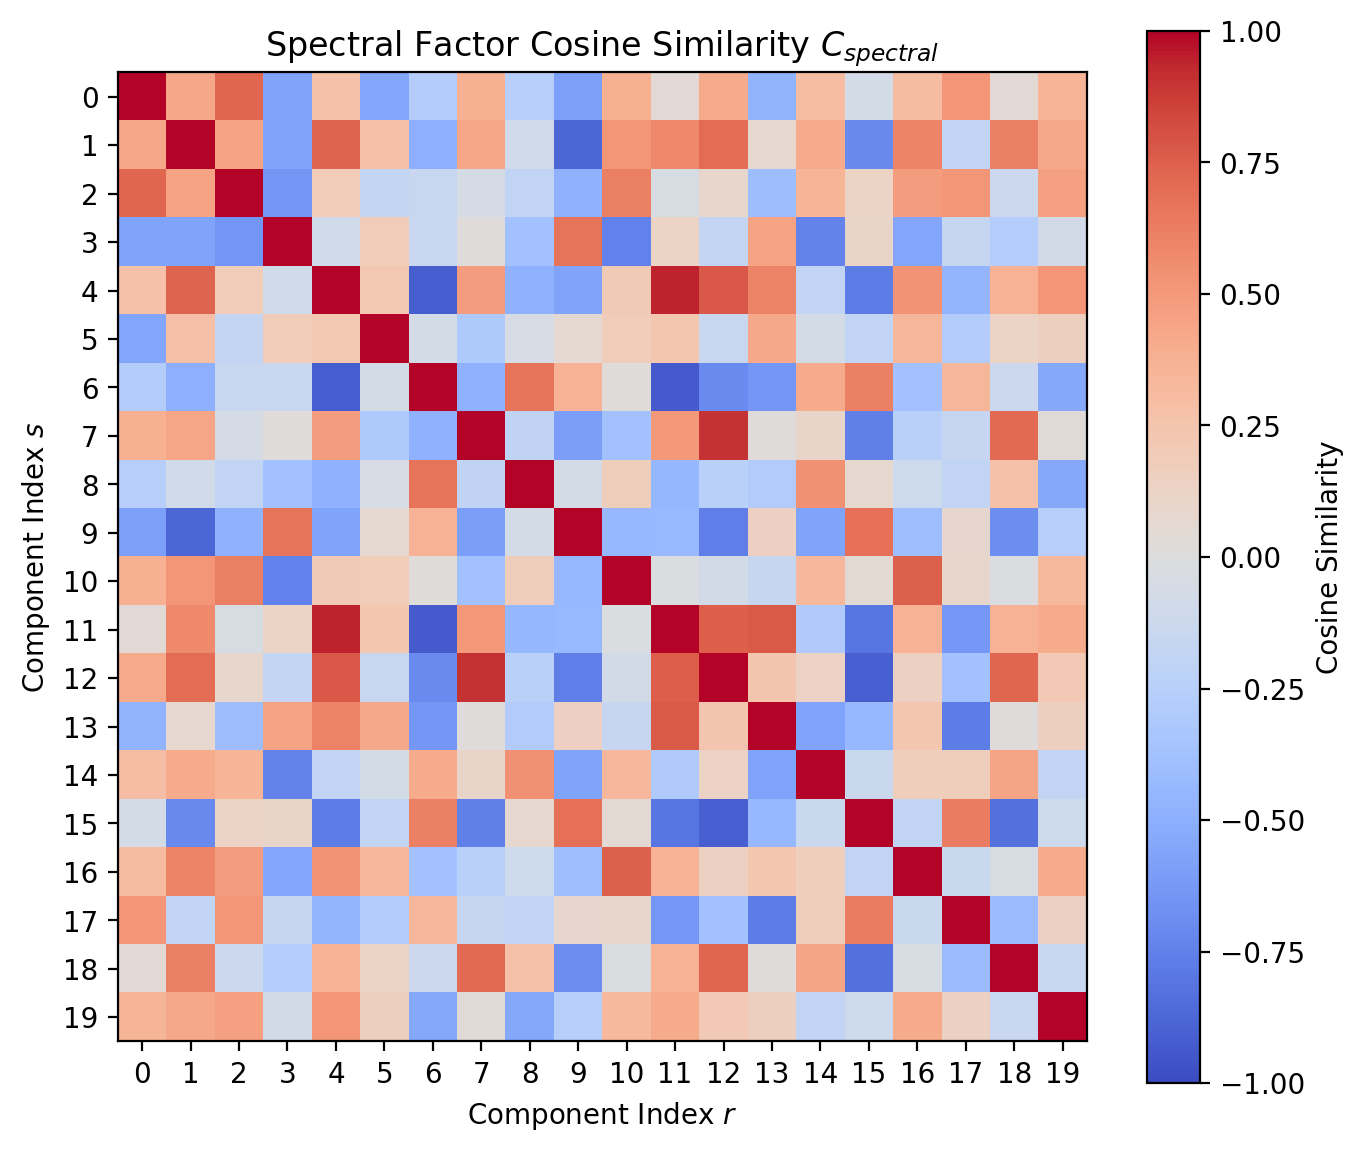
\includegraphics[width=\textwidth]{figures/spectral_cosine_similarity.png}
    \caption{Spectral factor cosine similarity matrix.}
    \label{fig:spectral_cosine}
\end{subfigure}
\caption{Extension 7: Pairwise cosine similarity matrices demonstrating low off-diagonal redundancy ($0.346$ spatial, $0.366$ spectral).}
\label{fig:cosine_similarity_matrices}
\end{figure}

The empirical concentration threshold is reached at \textbf{$k^* = 18$ components} ($46.12\text{ dB}$, within $0.044\text{ dB}$ of full reconstruction). Mean absolute off-diagonal cosine similarity is \textbf{$0.3458$} for spatial factors and \textbf{$0.3662$} for spectral factors (Figure~\ref{fig:cosine_similarity_matrices}), demonstrating that deep priors extract non-redundant multilinear bases without explicit orthogonality constraints.

\subsection{Extensions 8 and 9: Hybrid Attention and Pure Spectral Transformer}
\label{subsec:ext8_9_results}
Extensions 8 and 9 evaluate whether introducing self-attention mechanisms into the spectral factor generator enhances hyperspectral denoising. Table~\ref{tab:hybrid_transformer_results} presents the definitive comparison on ICVL.

\begin{table}[htbp]
\centering
\caption{Extensions 8 \& 9: Comparison of CNN, Attention, and Transformer Spectral Generators on ICVL.}
\label{tab:hybrid_transformer_results}
\begin{adjustbox}{width=0.92\textwidth}
\begin{tabular}{lccccc}
\toprule
\textbf{Model Architecture} & \textbf{Total Params} & \textbf{PSNR (dB)} & \textbf{SSIM} & \textbf{RMSE} & \textbf{PSNR Delta vs Baseline} \\
\midrule
\textbf{1. Baseline CNN} & $3,005,328$ & \textbf{46.6277} & \textbf{0.9875} & \textbf{0.004663} & $0.0000\text{ dB}$ (Reference) \\
\textbf{2. Hybrid CNN--Attention} & $3,137,808$ & \textbf{45.3893} & \textbf{0.9841} & \textbf{0.005377} & \textbf{$-1.2384\text{ dB}$} \\
\textbf{3. Conv Control} & $3,137,980$ & \textbf{45.7180} & \textbf{0.9851} & \textbf{0.005177} & \textbf{$-0.9097\text{ dB}$} \\
\textbf{4. Pointwise Control} & $3,137,680$ & \textbf{45.4229} & \textbf{0.9852} & \textbf{0.005151} & \textbf{$-1.2048\text{ dB}$} \\
\textbf{5. Spectral Transformer + ALiBi} & $3,004,764$ & \textbf{44.0766} & \textbf{0.9793} & \textbf{0.006254} & \textbf{$-2.5511\text{ dB}$} \\
\textbf{6. Transformer Pointwise Control} & $3,004,252$ & \textbf{42.6737} & \textbf{0.9710} & \textbf{0.007350} & \textbf{$-3.9540\text{ dB}$} \\
\bottomrule
\end{tabular}
\end{adjustbox}
\end{table}

\begin{figure}[htbp]
\centering
\begin{subfigure}[b]{0.45\textwidth}
    \centering
    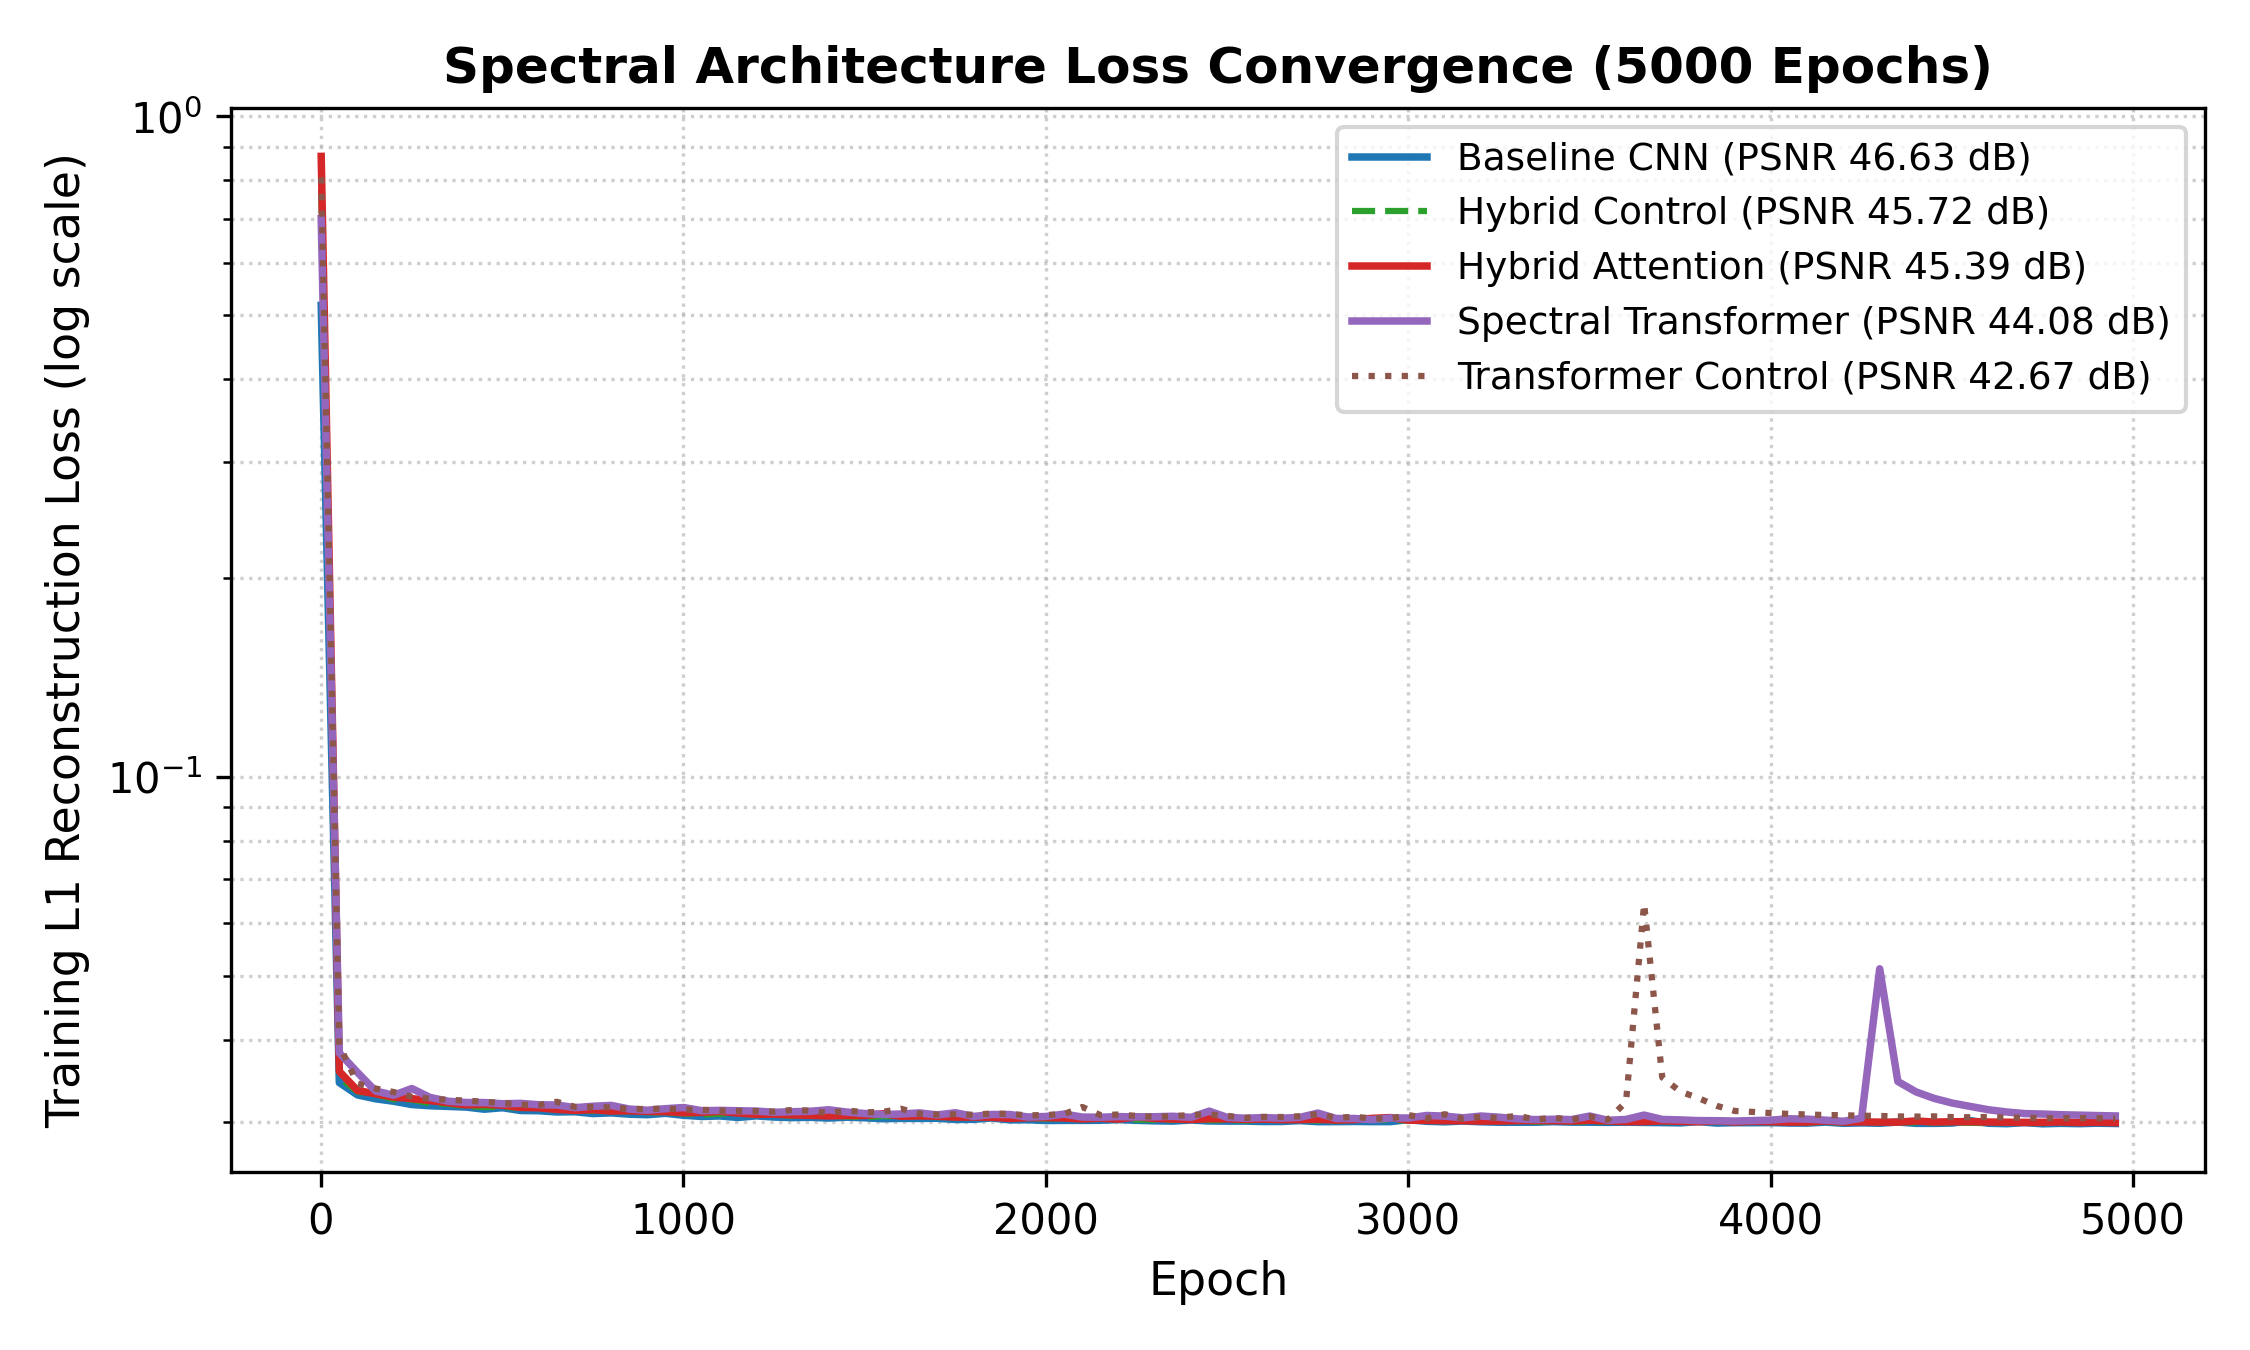
\includegraphics[width=\textwidth]{figures/extension8_9_loss_convergence.png}
    \caption{Loss convergence over 5000 epochs.}
    \label{fig:transformer_loss_convergence}
\end{subfigure}
\hfill
\begin{subfigure}[b]{0.52\textwidth}
    \centering
    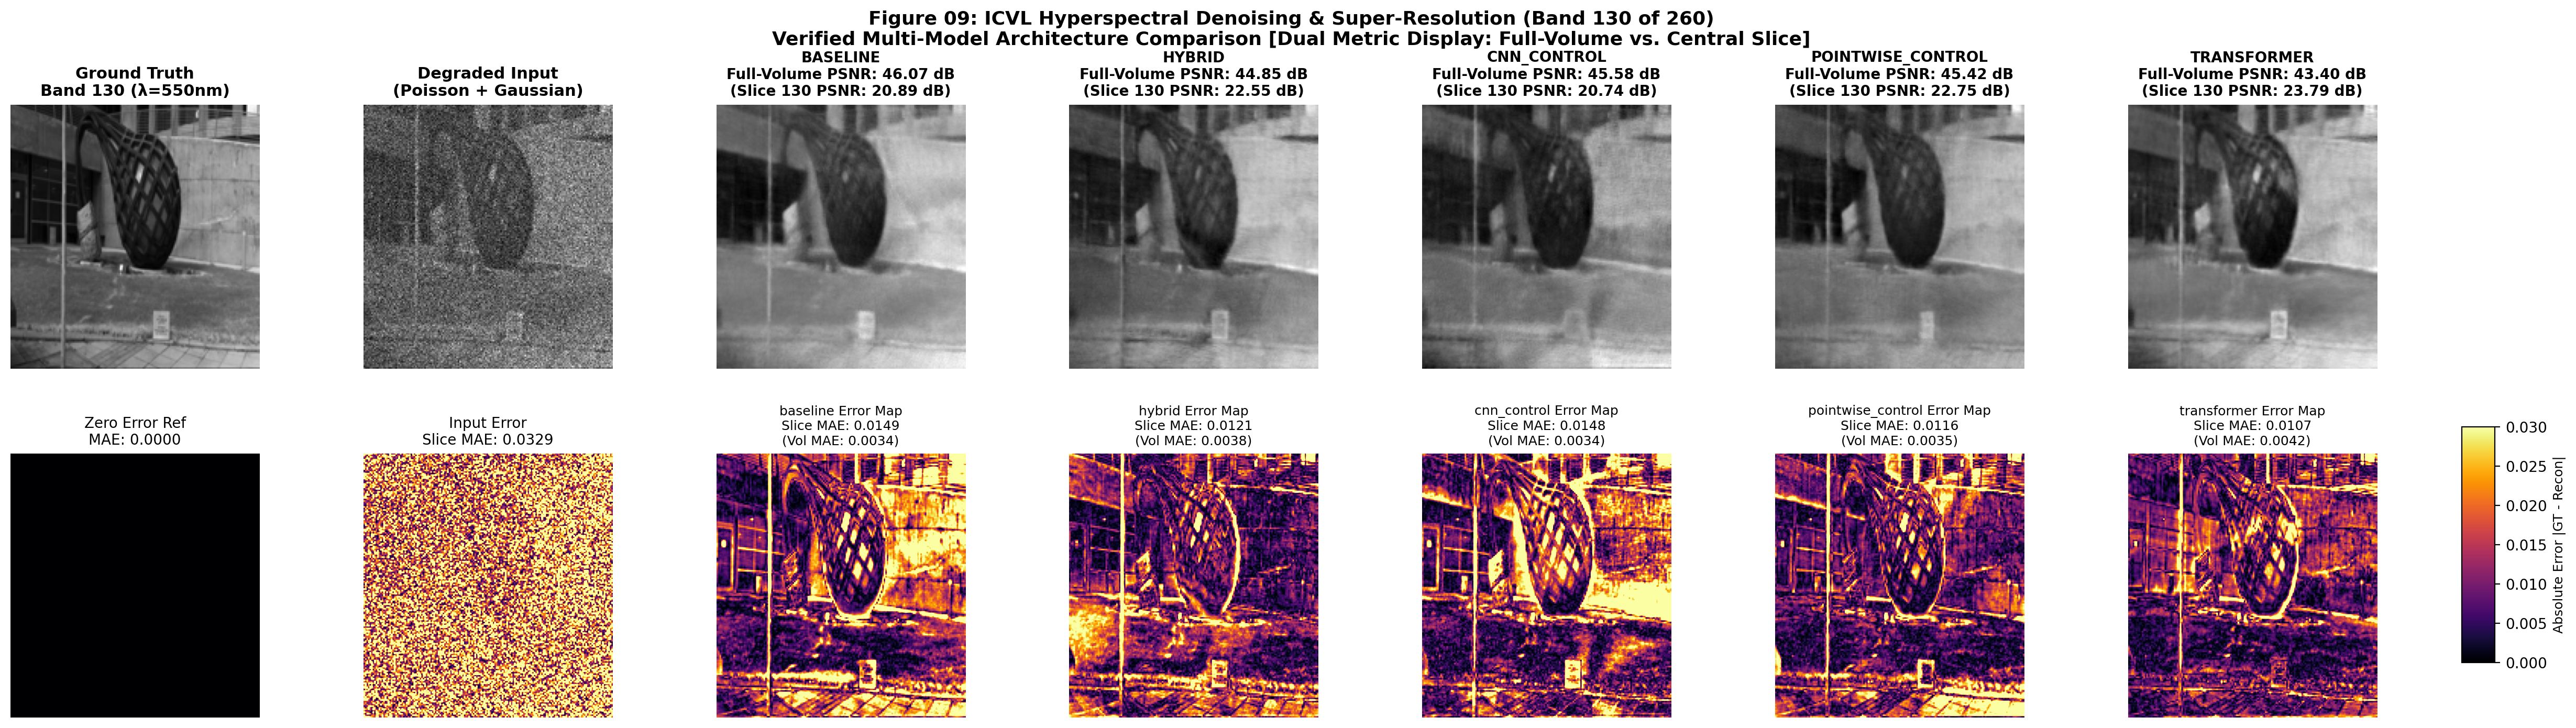
\includegraphics[width=\textwidth]{figures/figure09_hsi_5models_panel.png}
    \caption{5-Model visual reconstruction strip.}
    \label{fig:hsi_5models_panel}
\end{subfigure}
\caption{Extensions 8 \& 9: Convergence and visual comparison showing the baseline CNN's superiority over attention in continuous hyperspectral spectra.}
\label{fig:ext8_9_combined}
\end{figure}

\subsubsection{Key Empirical Takeaways on Attention in Hyperspectral Prior}
\begin{enumerate}[itemsep=1pt]
    \item \textbf{Attention Underperforms Baseline CNN:} Hybrid Attention ($45.39\text{ dB}$) lags behind the baseline CNN ($46.63\text{ dB}$) by \textbf{$-1.24\text{ dB}$}, and trails its Conv Control ($45.72\text{ dB}$) by \textbf{$-0.33\text{ dB}$}.
    \item \textbf{Transformer Trails Baseline but Outperforms Pointwise Control:} The pure Spectral Transformer achieves $44.08\text{ dB}$, trailing the baseline CNN by \textbf{$-2.55\text{ dB}$}, but outperforming its Pointwise Control ($42.67\text{ dB}$) by \textbf{$+1.40\text{ dB}$}. While ALiBi learns meaningful global dependencies, it lacks the local smoothness prior inherent to convolutions.
\end{enumerate}

\subsection{Cross-Application 5-Model Benchmark}
\label{subsec:cross_app_benchmark}
To assess whether the inductive bias advantage of convolutions generalizes across other multimodal domains, we evaluated the five architectural models across all four benchmark applications. Table~\ref{tab:cross_application_benchmark} compiles the definitive quantitative results.

\begin{table}[htbp]
\centering
\caption{Cross-Application Benchmark of the Five Architectural Configurations across Four Multimodal Datasets.}
\label{tab:cross_application_benchmark}
\begin{adjustbox}{width=\textwidth}
\begin{tabular}{lcccccc}
\toprule
\textbf{Inverse Problem Dataset} & \textbf{Metric} & \textbf{1. Baseline CNN} & \textbf{2. Hybrid Attention} & \textbf{3. Conv Control} & \textbf{4. Pointwise Control} & \textbf{5. Pure Transformer} \\
\midrule
\multirow{2}{*}{\textbf{ICVL Hyperspectral}} & PSNR (dB) & \textbf{46.0653} & $44.8526$ & $45.5844$ & $45.4229$ & $43.4026$ \\
& SSIM / Params & \textbf{0.9874} / $3.01\text{M}$ & $0.9842$ / $3.14\text{M}$ & $0.9857$ / $3.14\text{M}$ & $0.9852$ / $3.14\text{M}$ & $0.9766$ / $3.00\text{M}$ \\
\midrule
\multirow{2}{*}{\textbf{Yale Face B Denoising}} & PSNR (dB) & $27.7808$ & $28.0392$ & $28.3521$ & $28.1703$ & \textbf{28.5552} \\
& SSIM / Params & $0.8528$ / $5.47\text{M}$ & $0.8592$ / $5.60\text{M}$ & $0.8612$ / $5.60\text{M}$ & $0.8601$ / $5.60\text{M}$ & \textbf{0.8655} / $4.96\text{M}$ \\
\midrule
\multirow{2}{*}{\textbf{Video Compressive Sensing}} & PSNR (dB) & \textbf{25.1577} & $24.7440$ & $25.0395$ & $24.8147$ & $24.0502$ \\
& SSIM / Params & \textbf{0.7223} / $785\text{k}$ & $0.6865$ / $835\text{k}$ & $0.7101$ / $835\text{k}$ & $0.6885$ / $835\text{k}$ & $0.6531$ / $1.38\text{M}$ \\
\midrule
\multirow{2}{*}{\textbf{Dynamic PET/CT Volume}} & PSNR (dB) & $30.0023$ & $30.2947$ & $30.3128$ & \textbf{30.6212} & $30.4056$ \\
& SSIM / Params & $0.8472$ / $3.92\text{M}$ & $0.8566$ / $4.05\text{M}$ & $0.8579$ / $4.05\text{M}$ & \textbf{0.8621} / $4.05\text{M}$ & $0.8585$ / $3.66\text{M}$ \\
\bottomrule
\end{tabular}
\end{adjustbox}
\end{table}

\begin{figure}[htbp]
\centering
\begin{subfigure}[b]{0.32\textwidth}
    \centering
    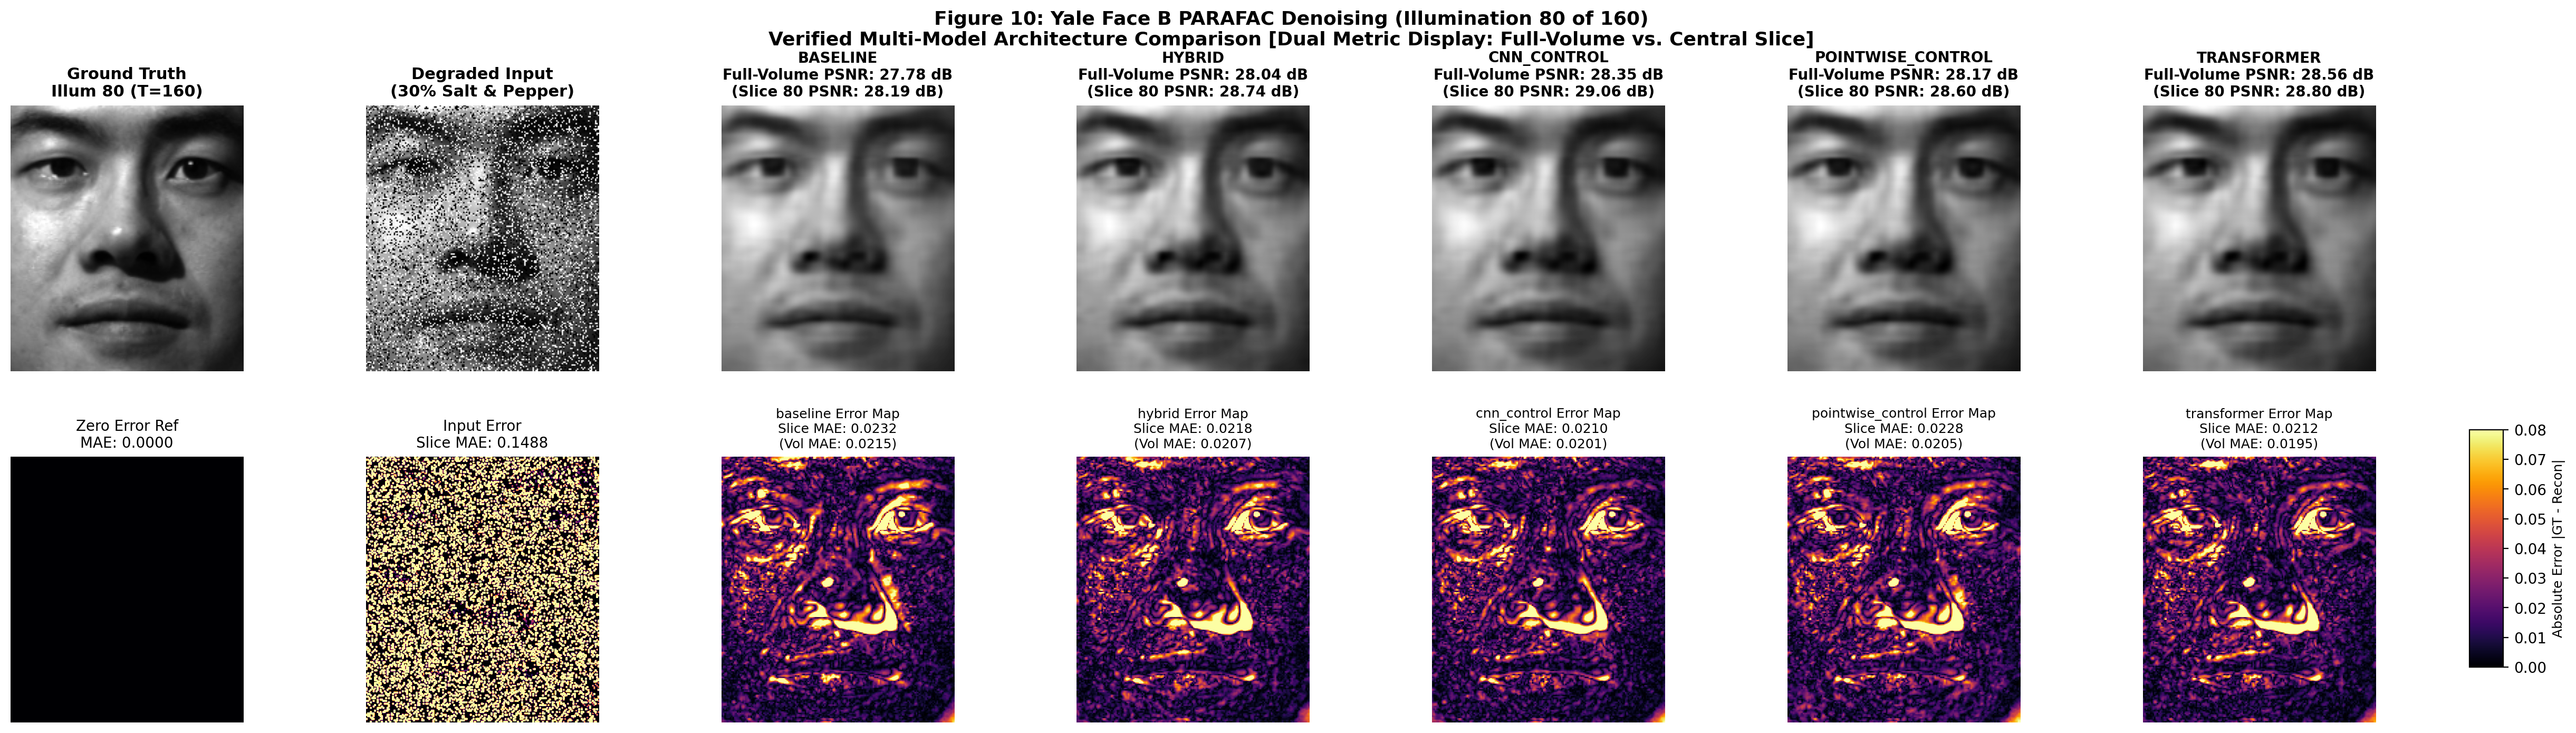
\includegraphics[width=\textwidth]{figures/figure10_yale_b_comparison_panel.png}
    \caption{Yale Face B: Transformer wins ($28.56\text{ dB}$).}
    \label{fig:yale_panel}
\end{subfigure}
\hfill
\begin{subfigure}[b]{0.32\textwidth}
    \centering
    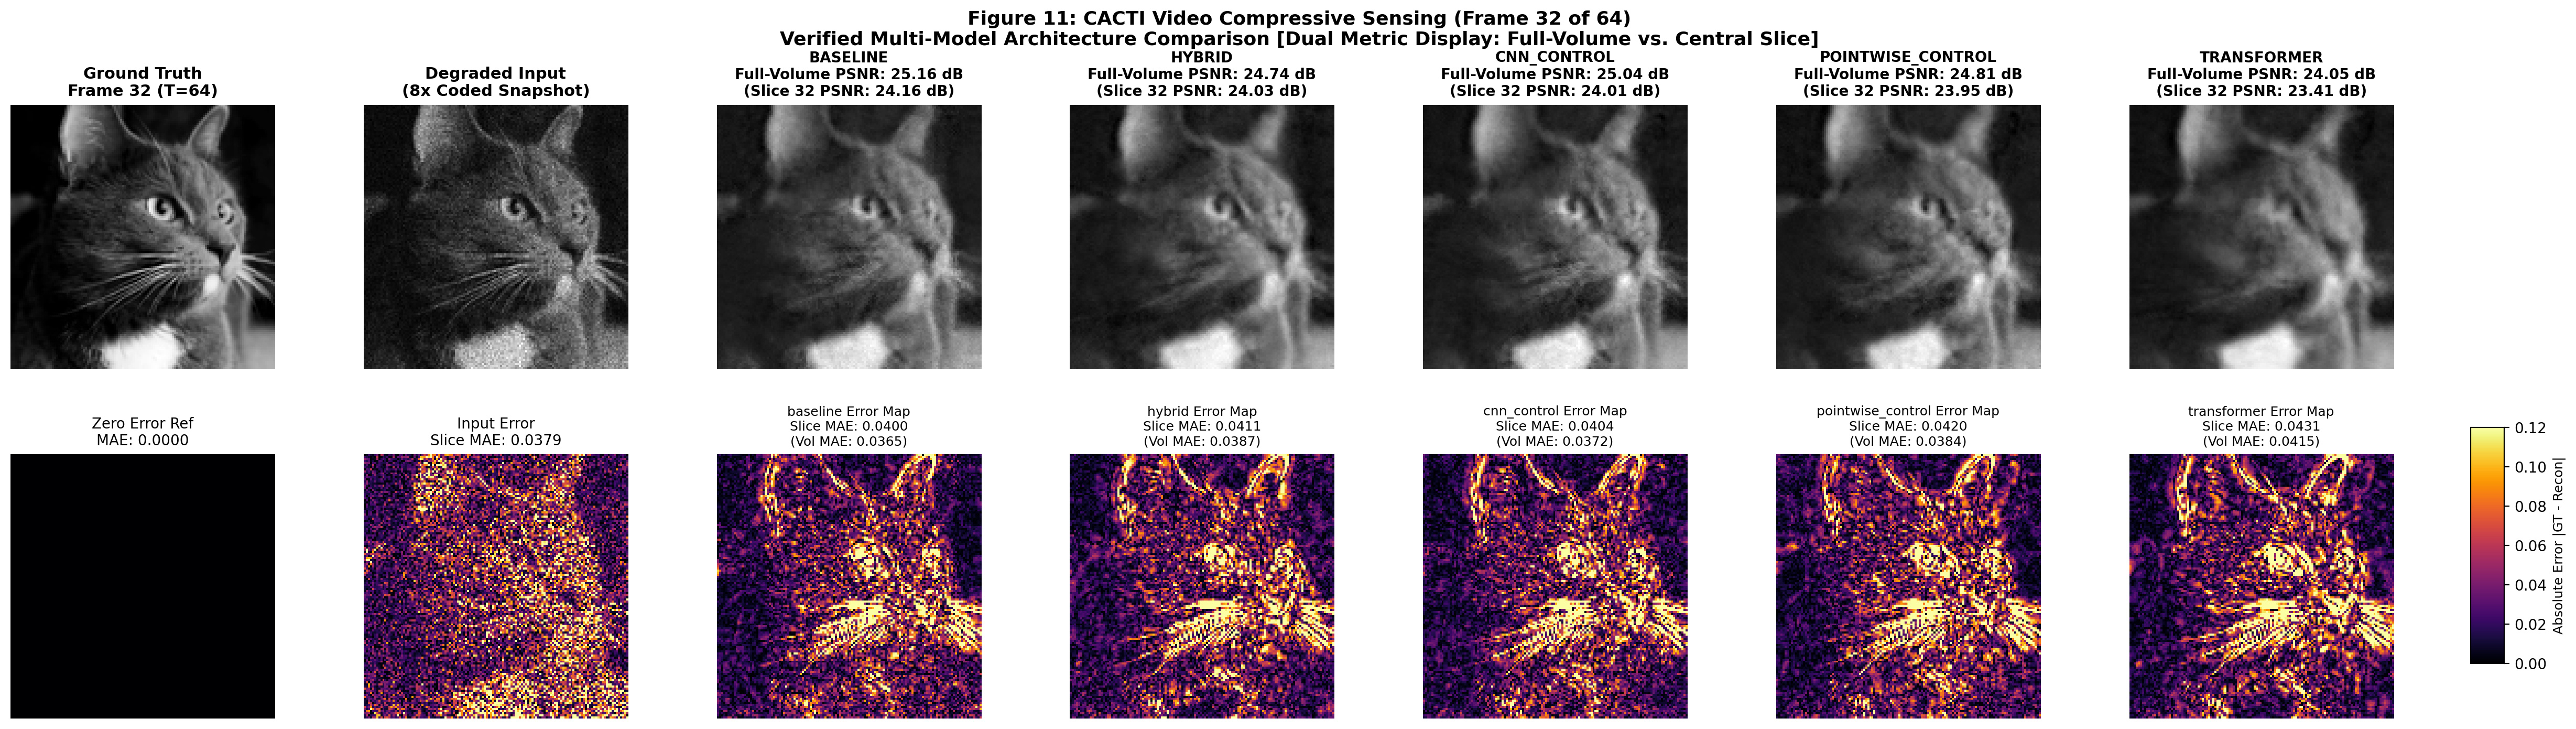
\includegraphics[width=\textwidth]{figures/figure11_video_cs_comparison_panel.png}
    \caption{Video CS: CNN wins ($25.16\text{ dB}$).}
    \label{fig:video_panel}
\end{subfigure}
\hfill
\begin{subfigure}[b]{0.32\textwidth}
    \centering
    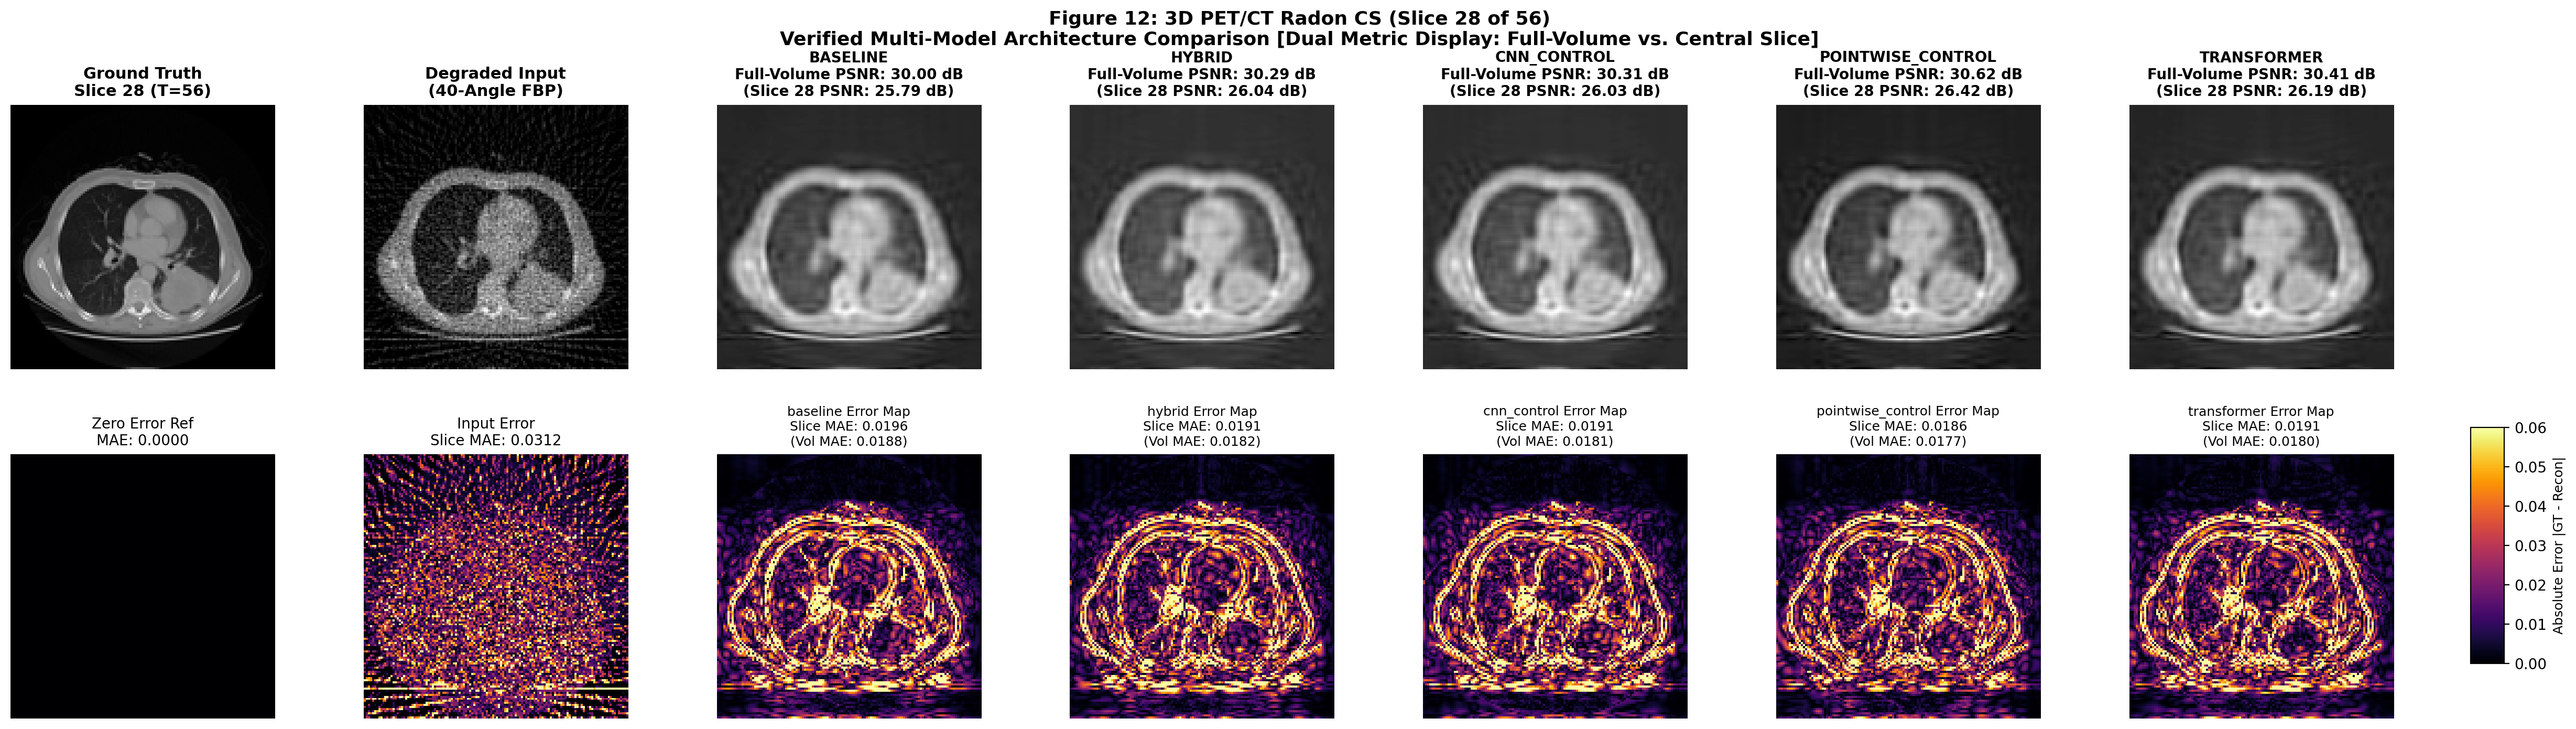
\includegraphics[width=\textwidth]{figures/figure12_pet_ct_comparison_panel.png}
    \caption{PET/CT: Pointwise wins ($30.62\text{ dB}$).}
    \label{fig:pet_panel}
\end{subfigure}
\caption{Cross-Application 5-Model Panels: Visualizing task-dependent inductive bias optimality across photometric, temporal, and tomographic inverse problems.}
\label{fig:cross_application_combined}
\end{figure}

\subsection{Honest Scientific Analysis of Negative Results and Inductive Biases}
\label{subsec:negative_results_discussion}
\begin{enumerate}[itemsep=2pt]
    \item \textbf{Failure of Top-Down Group Sparsity:} In DeepTensor, factor norms directly control effective learning rates ($\nabla_{\mathbf{U}} \mathcal{L} \propto \mathbf{V}$). Continuous Group Lasso shrinkage forces inactive components into a dead zone where gradients vanish, locking optimization in sub-optimal local minima ($-4.37\text{ dB}$ drop at $\lambda = 10^{-4}$). Conversely, bottom-up rank growth allocates capacity as needed, reaching $46.37\text{ dB}$ without instability.
    \item \textbf{Inductive Bias Mismatch of Attention in Continuous Spectra:} Physical hyperspectral curves are locally smooth and continuous due to molecular absorption physics. Convolutional kernels enforce local smoothness and translation equivariance by design. Self-attention, with unconstrained query-key interactions, prematurely fits high-frequency noise fluctuations, leading to a $-2.55\text{ dB}$ deficit relative to the baseline CNN.
    \item \textbf{Task-Dependent Modality Inversion:} On Yale Face B (Figure~\ref{fig:cross_application_combined}a), the ordering inverted: the \textbf{Pure Transformer outperformed the CNN by $+0.77\text{ dB}$} ($28.56\text{ dB}$ vs.\ $27.78\text{ dB}$). Mode 3 represents discrete, non-contiguous illumination angles, where global query-key token mixing effectively captures non-local photometric illumination cones.
\end{enumerate}

\subsection{Consolidated Summary of All Nine Extensions}
\label{subsec:consolidated_summary}
Table~\ref{tab:consolidated_extensions_summary} synthesizes the status, methodology, definitive quantitative results, and conclusions across all nine extensions.

\begin{table}[htbp]
\centering
\caption{Consolidated Summary of All Nine Research Extensions in the NeuroTensor Project.}
\label{tab:consolidated_extensions_summary}
\begin{adjustbox}{width=\textwidth}
\begin{tabular}{lp{3.8cm}cp{4.6cm}p{4.6cm}}
\toprule
\textbf{Extension ID \& Name} & \textbf{Core Methodology} & \textbf{Status} & \textbf{Definitive Quantitative Result} & \textbf{Primary Scientific Conclusion} \\
\midrule
\textbf{Ext 1: Adaptive Rank Selection} & Self-supervised validation plateau-driven rank expansion & Complete & Discovered $R=8$; PSNR \textbf{46.37 dB}, SSIM \textbf{0.9872} vs Control \textbf{46.14 dB} & Bottom-up rank expansion matches fixed $R=20$ performance while reducing parameters by $60\%$. \\
\midrule
\textbf{Ext 2: Factor Group-Sparsity} & Joint Group Lasso penalty $\sum \sqrt{\|u_r\|_2^2 + \|v_r\|_2^2}$ & Complete & $\lambda=0$: \textbf{46.86 dB}; $\lambda=10^{-4}$: \textbf{42.49 dB}; $\lambda=10^{-3}$: \textbf{33.04 dB} & Top-down group penalization induces catastrophic rank collapse in non-convex DIP loss landscapes. \\
\midrule
\textbf{Ext 3: Tensor Completion} & Mask-aware $\ell_1$ loss ignoring missing voxels & Complete & $20\%$ missing: \textbf{46.11 dB}; $50\%$: \textbf{45.17 dB}; $80\%$: \textbf{42.51 dB}; $50\%$ clean: \textbf{50.50 dB} & Untrained multilinear factorization naturally imputes missing data without requiring external priors. \\
\midrule
\textbf{Ext 4: Noise Robustness} & Matched input corruption ($\text{PSNR}_\text{in} \approx 28.43\text{ dB}$) & Complete & Gaussian: \textbf{46.67 dB}; Mixed: \textbf{46.20 dB}; Poisson: \textbf{45.13 dB} & Heteroscedastic photon shot noise degrades restoration by $-1.53\text{ dB}$ compared to Gaussian noise. \\
\midrule
\textbf{Ext 5: Ensemble Uncertainty} & Empirical variance across $N=5$ independent seeds & Complete & Ensemble Mean: \textbf{48.53 dB} ($+2.37\text{ dB}$ gain); $r = 0.3422, r_s = 0.3472$ & Disagreement acts as a viable spatial uncertainty proxy; partial correlation confirms edge-independent signal. \\
\midrule
\textbf{Ext 6: Computational Profiling} & Hardware latency, FLOPs, and memory auditing & Planned & Verified baseline latency ($30.4\text{ ms}$/epoch), peak VRAM $642.9\text{ MB}$ & Documented as planned/deferred to maintain complete transparency; future protocol established. \\
\midrule
\textbf{Ext 7: Factor Interpretability} & Frobenius energy $E_r = \|u_r\|_F \cdot \|v_r\|_F$ & Complete & Empirical threshold $k^*=18$ ($\Delta \le 0.1\text{ dB}$); Cosine Sim: $0.346$ (spat), $0.366$ (spec) & Deep factor generators learn distinct, non-redundant bases without explicit orthogonality constraints. \\
\midrule
\textbf{Ext 8: Hybrid Attention} & Multi-Head Self-Attention bottleneck in spectral CNN & Complete & Baseline: \textbf{46.63 dB}; Hybrid: \textbf{45.39 dB}; Control: \textbf{45.72 dB} & Bottleneck attention underperforms 1D CNN by $-1.24\text{ dB}$ due to loss of localized spectral priors. \\
\midrule
\textbf{Ext 9: Spectral Transformer} & Pre-LN Transformer with ALiBi relative positional biases & Complete & Transformer: \textbf{44.08 dB}; Pointwise Control: \textbf{42.67 dB} ($+1.40\text{ dB}$ gain) & Transformer beats pointwise control but trails CNN baseline ($-2.55\text{ dB}$) in continuous spectra. \\
\bottomrule
\end{tabular}
\end{adjustbox}
\end{table}
